%% Mars Global Mosaic: the final paper, AASTeX 7 (aastex701.cls).
%% Every number is quoted from Mars Remote Sensing Project\PROJECT-KNOWLEDGE.md (the KB) or the log it cites;
%% the KB section of each is kept in a comment beside it so it can be rechecked. Figures are copied into
%% figures\ by build\build_final_paper.py, which also compiles this file.
\documentclass[twocolumn]{aastex701}

\usepackage{amsmath}

\newcommand{\pmsixty}{$\pm60^{\circ}$}
\newcommand{\kap}{$\kappa$}
\newcommand{\lAv}{\textit{lAv}}

\shorttitle{Mars Global Mosaic}
\shortauthors{Edwards}

\begin{document}

\title{Mars Global Mosaic: Mapping Lava Flows, Fluvial Channels, and Impact Craters in Visible and Infrared}

\author{Logan M Edwards}
\affiliation{Florida Institute of Technology, OCN 4704 Remote Sensing, Melbourne, FL 32901, USA}
\email{ledwards2024@my.fit.edu}

\begin{abstract}
Viking MDIM~2.1 visible colour, THEMIS day and night thermal-infrared mosaics and the HRSC/MOLA blended elevation
model were co-registered on one 100~m and 200~m grid spanning \pmsixty\ latitude, 86.6\% of Mars, to map impact
craters, fluvial channels and lava flows. At Ius Chasma the visible bands are one dimension ($r=0.93$--$0.99$)
and night infrared is nearly independent of every band ($|r|\le0.12$). Across \pmsixty, however,
the THEMIS mosaics are 8-bit products stretched region by region: dusty and rocky provinces differ by 47.67~DN in
Viking red but by $-0.19$ and $+0.02$~DN in day and night infrared, and against calibrated TES thermal inertia the
THEMIS pair keeps only a weak local signal ($|r|\approx0.1$) while Viking albedo tracks inertia planet-wide
($r=-0.36$). Fill depth yields 465,354 closed depressions $\ge1$~km; 62.2\% of those $\ge5$~km are catalogued
craters, only 15.3\% at $\ge1$~km, and breached craters are invisible to the method. Of 969,822 routed channel
segments 89.8\% lie on slopes under $2^{\circ}$, and stream order follows the accumulation threshold, not the
terrain. A support vector machine trained on 512 hand-drawn landform polygons and scored on whole $15^{\circ}$
blocks it never saw reaches 73.8\%, \kap\,0.58 (one class everywhere: 58.6\%); the thermal bands add a resolved 1.4
to 2.0 points. A U-Net reaches 98.9\% on the same blocks as a terrain-province map. No band separates the lava
contacts of the 1:20\,M geologic map at Athabasca Valles much better than chance, so lava flows are taken from
that map. Three of four hypotheses are not supported; the fourth was answered by another method.
\end{abstract}

\keywords{Mars --- Planetary surfaces --- Remote sensing --- Infrared imaging --- Impact craters --- Lava flows ---
Fluvial geomorphology --- Machine learning}

%% ====================================================================================================
\section{Introduction} \label{sec:intro}

Athabasca Valles, a young channel system south of Elysium, was read for decades as an outflow channel carved by
water released from the Cerberus Fossae \citep{Burr2002, Plescia2003}. High-resolution imaging later showed the
channel floor draped by a single turbulent flood of lava \citep{Jaeger2007, Jaeger2010}, and the USGS geologic map
places it in the Late Amazonian volcanic unit \lAv\ \citep{Tanaka2014}. The case makes the question of this project
concrete: can a co-registered visible and thermal-infrared mosaic separate lava, water and impact landforms, and how
much of the answer comes from the thermal infrared? %% KB §14.4, §41

Thermal infrared is the natural candidate. Rock and coarse debris hold heat through the night while dust cools
quickly, so the diurnal temperature contrast follows thermal inertia, a property of particle size and induration
\citep{Mellon2000, Fergason2006, Putzig2007}. Visible albedo also separates bright dust from dark basalt
\citep{Ruff2002}, and topography carries the morphology of craters, channels and flow fronts. The global mosaics that
hold each of these quantities have been available for years \citep{Archinal2003, Edwards2011, Fergason2018}, but
they come on three different coordinate frames, and a usable stack of them is not a given.

This paper reports the stack, the landform products made from it and the tests run on them. The goals were (1) one
co-registered stack of Viking visible colour, THEMIS day and night infrared and HRSC/MOLA topography on a single grid;
(2) maps of the three landform families, first in a type area and then across the whole extent; (3) a test of whether
the thermal infrared separates surfaces that visible light cannot; and (4) a score for every product against
something it never saw. Four hypotheses were set when the project was proposed: H1, that day infrared shows
lava-flow margins under dust that Viking misses; H2, that fluvial channels have shallower gradients than volcanic ones
and the two separate on gradient against thermal response; H3, that the multi-band composite gives more stable
unsupervised classes than any single input; and H4, that crater rims found from image gradients recover most of the
141 named craters larger than 100~km. Each test below wrote its prediction and verdict rule into its script before it
ran. %% KB §14.1, §47, §51.1

%% ====================================================================================================
\section{Data} \label{sec:data}

\subsection{The source mosaics}

Four global or near-global products were used (Table~\ref{tab:data}). The THEMIS mosaics \citep{Christensen2004,
Edwards2011} are single-band 8-bit display products: the night mosaic's label gives a base of 0 and a multiplier of 1,
with no scaling to radiance or temperature, and the two mosaics were stretched independently (2nd and 98th percentiles
of 35 and 205~DN by day, 58 and 203~DN by night over Ius Chasma). Calibrated thermal inertia cannot be derived from
them. Viking MDIM~2.1 has every one of its 4.25 billion pixels valid; the HRSC/MOLA blend
\citep{Smith2001, Jaumann2007, Fergason2018} is signed 16-bit metres on a geographic grid. %% KB §3, §24.1

\begin{table*}[t]
\centering
\caption{The source mosaics, as held \label{tab:data}}
\small
\setlength{\tabcolsep}{4.5pt}
\begin{tabular}{lcccl}
\hline\hline
Product & Cell & Size (px) & Frame & Holds \\
\hline
Viking MDIM 2.1 colour & 231.5 m & $92{,}160\times46{,}080\times3$ & cylindrical, CM $0^{\circ}$ & visible albedo, RGB \\
THEMIS Day IR v12 & 100 m & $213{,}390\times106{,}696$ & cylindrical, CM $180^{\circ}$ & day brightness, 8-bit \\
THEMIS Night IR v14 & 100 m & $213{,}388\times71{,}130$ & cylindrical, CM $180^{\circ}$, \pmsixty & night brightness, 8-bit \\
HRSC/MOLA blend DEM v2 & $0.0033741^{\circ}$ & $106{,}694\times53{,}347$ & geographic, degrees & elevation, $-8.5$ to $+21.2$ km \\
\hline
\end{tabular}
\par\vspace{3pt}\noindent\parbox{\textwidth}{\footnotesize Note: THEMIS 6.8--14.9~$\mu$m. All four are uncompressed and stored one scanline per block; together about 62~GB. The DEM cell is 199.99999~m on the 3,396,190~m sphere.}
\end{table*}
%% KB §3, §15, §28.2, §45

\subsection{Reference data}

Four independent references score the products \citep{Congalton1991}. The USGS Geologic Map of Mars, SIM~3292
\citep{Tanaka2014}, supplies 1,311 unit polygons and is the lava-flow reference. The Robbins and Hynek database
\citep{Robbins2012}, 2020 release, holds 385,049 craters $\ge1$~km. TES thermal inertia \citep{Putzig2007}, dayside and
nightside at 20 pixels per degree, is the only calibrated thermal product. The IAU gazetteer \citep{Gazetteer} names
141 craters larger than 100~km. Every IAU crater larger than 100~km matches a Robbins crater with a median centre
offset of 1.0\% of its diameter, and the Athabasca Valles floor falls in unit \lAv\ of the geologic map, as
published. %% KB §41, §6

\subsection{The analysis extent and the type areas}

No global THEMIS night mosaic exists: coverage stops at $\pm60^{\circ}$. The analysis stack was therefore bounded at
\pmsixty, which removes a third of the rows of a simple cylindrical grid but only 13.4\% of the surface: 86.6\% of
Mars lies within \pmsixty. Relief inside the band equals global relief (29,343~m, Hellas Planitia to Olympus Mons); the
polar layered deposits and ice caps, none of them a target landform, are lost. Two type areas prove methods before
they run at \pmsixty: Ius Chasma ($271$--$286^{\circ}$E, $6$--$13^{\circ}$S), a canyon with the Louros Valles
tributaries, and Athabasca Valles ($150$--$162^{\circ}$E, $4$--$14^{\circ}$N), the flood lava (Figures~\ref{fig:locator}
and \ref{fig:athabasca}). %% KB §14.3, §15.4, §16, §42.1

\begin{figure*}[t]
\centering
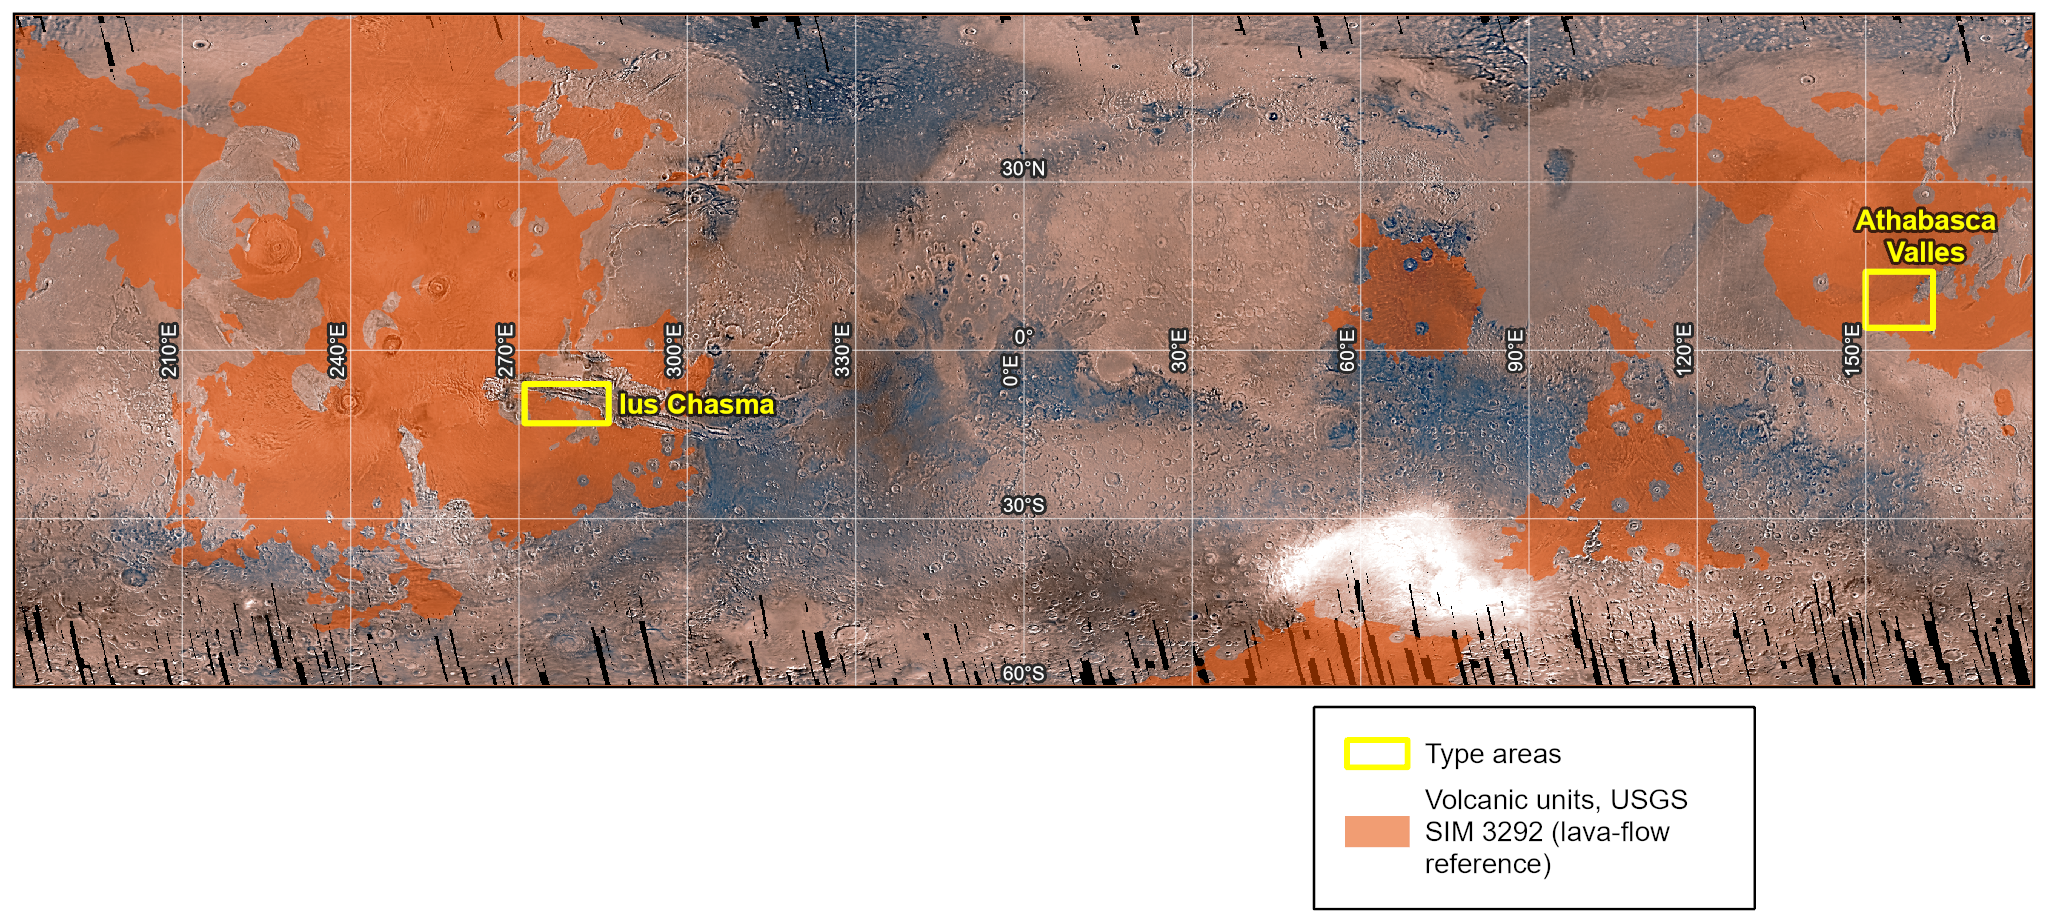
\includegraphics[width=\textwidth]{figures/10_global60_locator.png}
\caption{The analysis extent (\pmsixty) over Viking MDIM~2.1 colour, the two type areas, and the volcanic units of the
USGS geologic map SIM~3292 \citep{Tanaka2014} in orange, the lava-flow reference of this study. Geographic
coordinates, centred on $0^{\circ}$E. \label{fig:locator}}
\end{figure*}

\begin{figure*}[t]
\centering
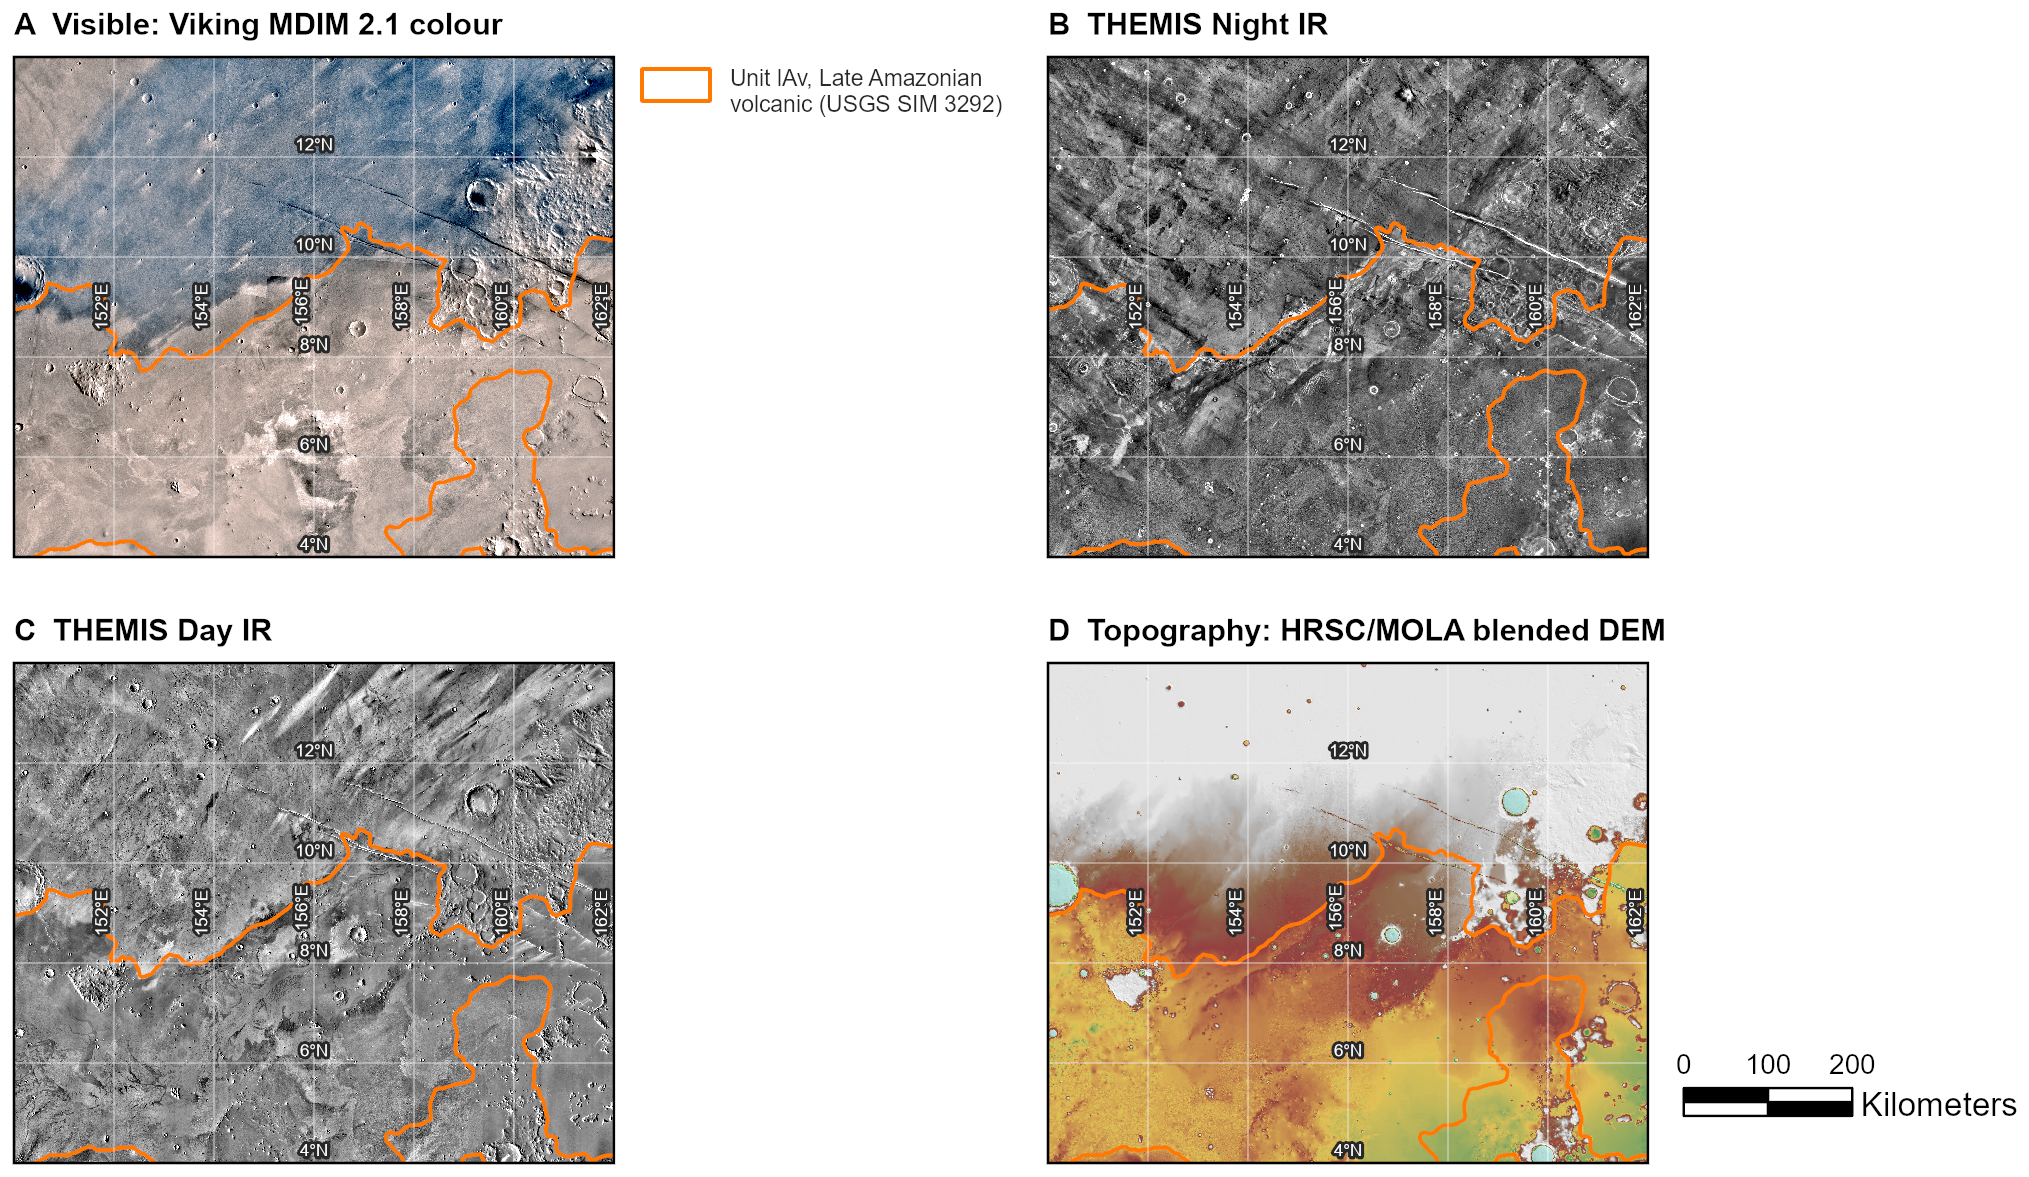
\includegraphics[width=0.92\textwidth]{figures/15_athabasca_type_area.png}
\caption{The Athabasca Valles type area on the 100~m stack: (A) Viking colour, (B) THEMIS night infrared, (C) THEMIS
day infrared, (D) the HRSC/MOLA elevation model ($-4{,}495$ to $1{,}945$~m) over hillshade. The orange outline is unit
\lAv, Late Amazonian volcanic, of SIM~3292. \label{fig:athabasca}}
\end{figure*}

%% ====================================================================================================
\section{Methods} \label{sec:methods}

All processing ran headless through \texttt{arcpy} in ArcGIS Pro~3.7 \citep{ArcGISPro}, with GDAL \citep{GDAL} and
NumPy \citep{Harris2020} for raster arithmetic, on a workstation with an Intel i7-8700K, 64~GB of memory and an NVIDIA
RTX~2080~Ti; figures were drawn with Matplotlib \citep{Hunter2007} or exported from the project's map layouts. Every
product and figure has a script that regenerates it \citep{Edwards2026data}. %% KB §2.1, §2.4, §12.1

\subsection{Co-registration on one grid}

The four sources span three frames: THEMIS on a central meridian of $180^{\circ}$ (longitudes $0$--$360^{\circ}$E),
Viking on $0^{\circ}$ ($-180$ to $180^{\circ}$E), and the DEM in geographic degrees. A THEMIS window read at face value
lands half a planet away, and elevation derivatives computed on the degree grid carry an undefined vertical factor. A
global Composite Bands run on the unharmonised sources was cancelled four times by 13 September (and a fifth time on 24
September); projected first and bounded to the type area, the same composite took 8.8~s. %% KB §4, §8, §18

The common grid is read from the night mosaic itself: equidistant cylindrical, central meridian $180^{\circ}$, sphere
radius 3,396,190~m \citep{Archinal2018}, at 100~m (G100, $213{,}388\times71{,}130$, 15.18 billion pixels) and as its
exact $2\times2$ aggregation at 200~m (G200, $106{,}694\times35{,}565$). The day mosaic sits on the night grid at an
offset of exactly $+1$ and $+17{,}783$ pixels, so neither THEMIS mosaic is ever resampled. The DEM cell is
199.99999~m on this sphere, so a nearest-neighbour warp to G200 reproduces 262,144 of 262,144 sampled source pixels
exactly, where a cubic warp alters 36\% of them by up to 28~m; terrain is therefore computed on G200 and imagery on
G100. Slope, aspect and hillshade are computed in metres on the projected grid, which removes the vertical-factor
warning of the degree-grid products. %% KB §28.1, §28.2, §20

The DEM's last column proved defective (nodata in 24,335 rows and wrong values elsewhere; the file also ends 0.46
pixel short of $+180^{\circ}$), which painted a 2~km stripe of spurious classes along $180^{\circ}$. It was replaced
by the mean of its two neighbours and the affected products were recomputed over that column only. %% KB §54

\subsection{The classification stack}

The seven-band stack for classification is on G200 with 97.33\% of pixels valid in every band: Viking R, G and B
(bilinear from 231.5~m), THEMIS night and day infrared ($2\times2$ averages on their own grid), slope in degrees, and
local relief in a $9\times9$ window (1.8~km). Every band is stretched from its 1st and 99th percentiles over \pmsixty\
to 1--255. Elevation itself is excluded: a raw elevation band beside 8-bit bands dominates any distance-based classifier,
and an earlier map built with one was 62\% reproducible from elevation alone. %% KB §31.2, §30.3, §14.2

\subsection{The diurnal-contrast index}

Since calibrated inertia is unavailable, a relative index was formed: each THEMIS band is scaled by its own 2nd and
98th percentiles to $[0,1]$ and night is subtracted from day, giving a dimensionless value in $[-1,1]$ that is high for
a large diurnal swing (dust-like) and low for a damped one (rock and coarse debris). It is valid only within the area
over which it was stretched. Over Ius Chasma its mean is $+0.0757$ (s.d.\ 0.279), and it is nearly independent of
topography ($r=+0.108$ with elevation, $-0.248$ with slope). %% KB §24.2, §24.3

\subsection{Closed depressions and channels}

The \texttt{Fill} operation \citep{Jenson1988} floods every closed depression, which is what a fresh crater is
topographically, so fill depth is a crater detector. A depression is kept if it is deeper than 20~m, at least 1~km
across (about ten 100~m pixels, the resolving rule used throughout), no more than twice as long as wide, and fills at
least 0.55 of its bounding box. The thresholds were tuned on two named craters near Ius Chasma: Perrotin (82.8~km) is
found at 77.0~km ($-7.1\%$) and ranks first of 1,321 candidates; Oudemans (124.2~km) is missed, because it is breached
into the canyon and its lowest rim point lies 33~m below its floor. Across \pmsixty\ the detector runs at two scales:
the whole extent at 1.6~km for basins $\ge20$~km, and 8,192-pixel tiles of G200 with a 1,024-pixel (205~km) halo for
depressions $\ge1$~km. %% KB §26.2, §26.3, §26.4, §28.6

Channel centrelines come from D8 flow routing on the filled surface \citep{Jenson1988} with a 5,000-cell (50~km$^2$)
accumulation threshold, ordered after \citet{Strahler1957}. Because \texttt{Fill} turns closed basins into synthetic
lakes, only stream cells where the fill raised the surface by at most 1~m are kept. %% KB §25.1, §25.2

\subsection{Supervised classification and its score}

Five hundred and twelve polygons were drawn by hand in four landform classes across the planet: 302 Crater, 44 steep or
windy hills, 44 lava tube and 122 Normal Ground. Clipped to \pmsixty, they were split by whole $15^{\circ}\times15^{\circ}$
blocks (14 of 39 blocks held out) into 329 training and 183 held-out polygons, each polygon whole and assigned to the
block holding its centre \citep{Roberts2017}; one held-out polygon overlaps a training one by 51.5~km$^2$ across a
block edge. A support vector machine \citep{Cortes1995} was trained on the
training polygons (1,000 samples per class) and applied to all of \pmsixty\ at 200~m in 21 tiles of 16,384 pixels.
%% KB §29.2, §31.3, §54.3, §68.2, §68.5

Accuracy is the area-weighted (by $\cos$ latitude) share of held-out polygon area given its own class, with Cohen's
\kap\ \citep{Cohen1960} and per-class producer's and user's accuracy \citep{Congalton1991}. Because one class dominates
the held-out area, each map is also given its balanced accuracy (the mean producer's accuracy), the mean of the
per-class F1 scores, and its disagreement split into quantity (the wrong amount of a class) and allocation (the right
amount in the wrong place) after \citet{Pontius2011}. Three baselines accompany
every score: one class everywhere (58.6\% on the held-out set), the share of the map that elevation alone reproduces
(each 500~m bin given its majority class), and the share of named craters $\ge5$~km labelled Crater inside $0.7R$
against a ring at $1.5$--$2.5R$. A majority filter removes speckle; its window was set from the resolving rule (about
2~km) rather than from the score, because every score rises with every window when the labelled polygons are large.
%% KB §31.3, §30.1, §32.2, §57

\subsection{Deep learning}

Two models were trained on the training blocks only and scored on the same held-out polygons. A RetinaNet detector
\citep{Lin2017} with a ResNet-50 backbone \citep{He2016} was trained on 3,622 chips of $256\times256\times7$ pixels
(stride 128) holding 5,293 boxes; its score is per polygon, recall being the share of held-out polygons at least half
covered by boxes of their own class. A U-Net \citep{Ronneberger2015} with a ResNet-34 backbone, class balancing and
unlabelled ground ignored in the loss, was trained for 30 epochs on the same chips as pixel labels, applied to all of
\pmsixty\ in 243 tiles of 4,096 pixels with a 256-pixel margin, and scored with the same code as the support vector
machine. Because the classification tool works internally in 256-pixel tiles, the U-Net was run a second time on a grid
offset by 128 pixels, and each pixel was taken from the pass that places it farther from a tile edge. Both models used
the Deep Learning Libraries of ArcGIS Pro, built on PyTorch \citep{Paszke2019}. %% KB §50.2, §51.3, §66.1, §66.6, §66.7, §66.8

\subsection{Uncertainty}

Intervals are 95\% paired bootstrap intervals \citep{Efron1993} over whole held-out polygons (1,000 resamples), over
contacts for the flow-margin test and over 50~km cells for the channel test, so that spatially correlated pixels are
never treated as independent.

%% ====================================================================================================
\section{Results} \label{sec:results}

\subsection{The mosaic and the case for fusion}

Figure~\ref{fig:mosaic} shows the four layers on the common grid. Over Ius Chasma all five bands are valid on 100\% of
pixels, and their correlations (Table~\ref{tab:corr}) give the measured case for the fusion: the three Viking bands are
one dimension, day infrared is anticorrelated with visible ($r\approx-0.49$; bright dust is cool by day), and night
infrared is the most independent band. The effective dimensionality is about three. At Athabasca Valles the pattern
repeats (night $|r|\le0.15$ against every band). At \pmsixty\ the registration was confirmed between Viking red and day
infrared: the strongest correlation within $\pm19$~km lies at zero shift ($r=-0.147$), and none survives a
$180^{\circ}$ roll. %% KB §18.3, §42.1, §31.2

\begin{figure*}[t]
\centering
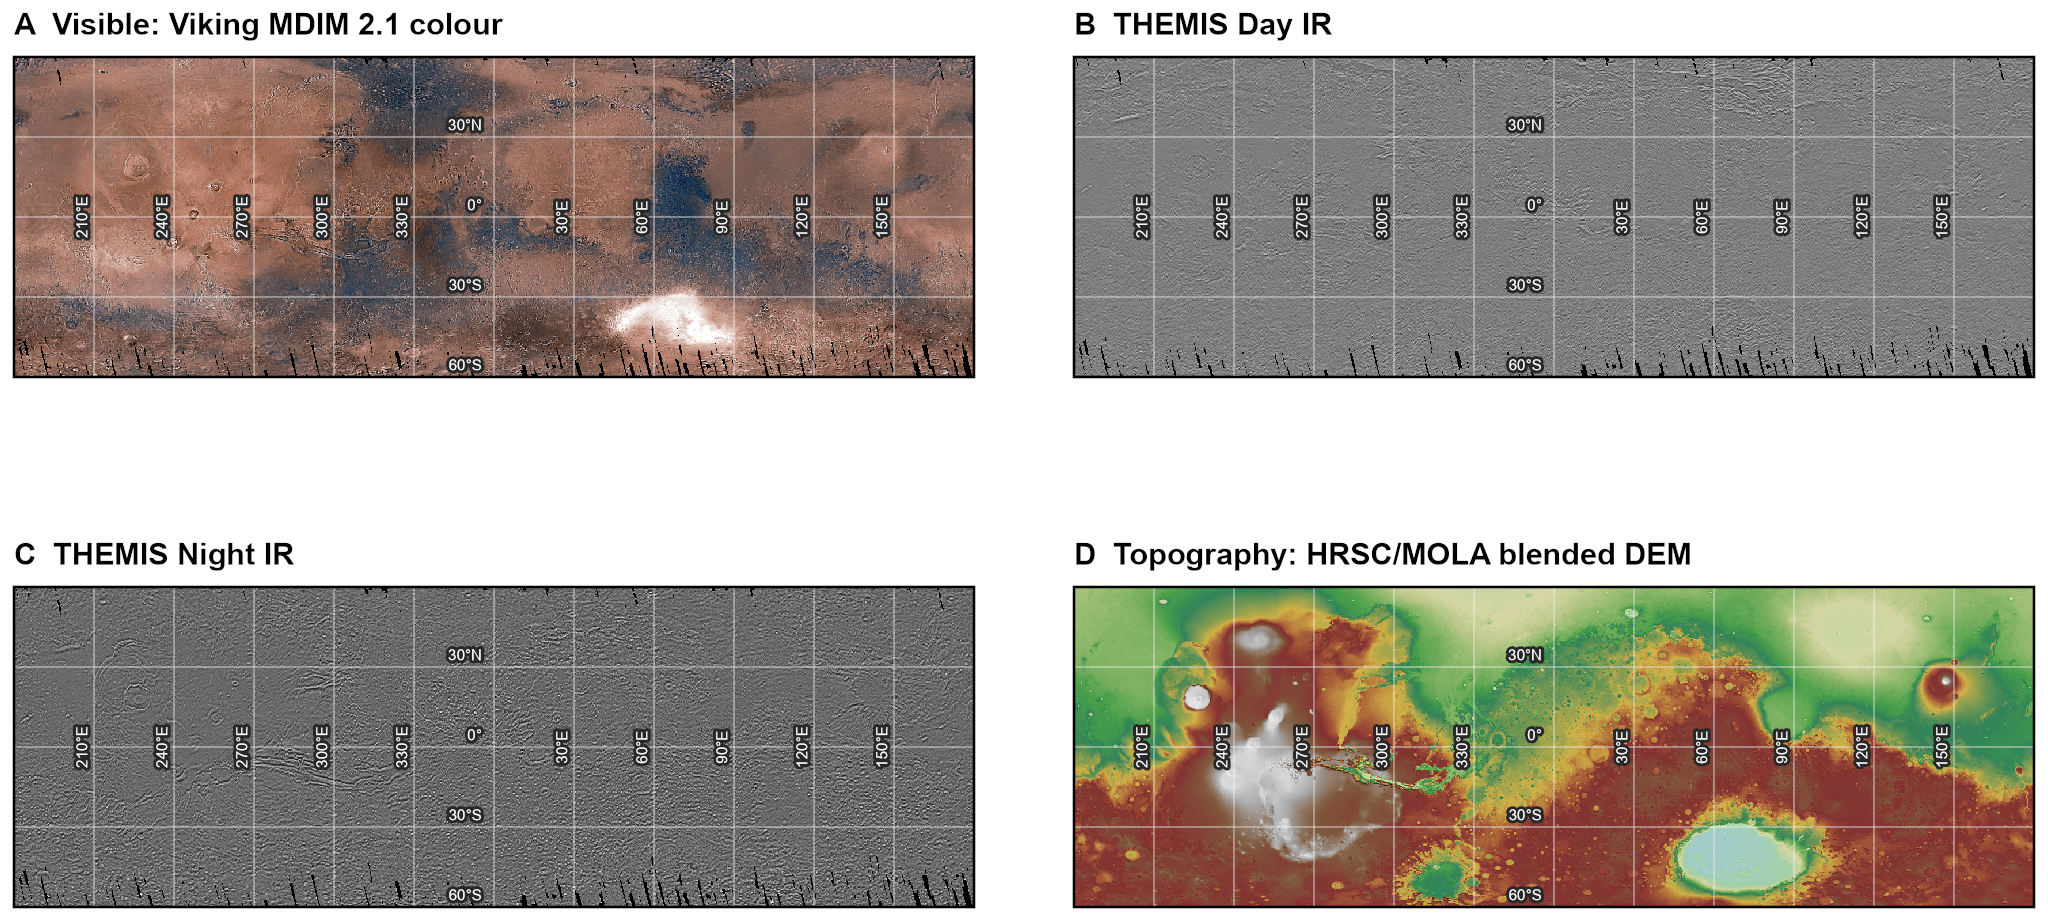
\includegraphics[width=\textwidth]{figures/08_global60_mosaic.png}
\caption{The co-registered mosaic at \pmsixty, drawn from the 200~m stack: (A) Viking visible colour, (B) THEMIS day
infrared, (C) THEMIS night infrared, (D) HRSC/MOLA topography over hillshade. Both THEMIS panels look nearly uniform at
this scale because the mosaics are contrast-stretched region by region (Section~\ref{sec:thermal}). \label{fig:mosaic}}
\end{figure*}

\begin{table}[t]
\centering
\caption{Band correlation over Ius Chasma ($8{,}891\times4{,}150$ pixels at 100~m) \label{tab:corr}}
\small
\begin{tabular}{lccccc}
\hline\hline
 & R & G & B & Day & Night \\
\hline
Viking R & 1 & 0.960 & 0.925 & $-0.486$ & $-0.121$ \\
Viking G & & 1 & 0.993 & $-0.496$ & $-0.085$ \\
Viking B & & & 1 & $-0.488$ & $-0.068$ \\
Day IR & & & & 1 & 0.105 \\
Night IR & & & & & 1 \\
\hline
\end{tabular}
\end{table}
%% KB §18.1, §18.3

\subsection{What the thermal pair can and cannot do} \label{sec:thermal}

Inside one area the diurnal-contrast index behaves as a material signal should. On the object-based classes of Ius
Chasma the steep canyon wall (mean slope $21.5^{\circ}$) and the mantled chasma floor ($17.0^{\circ}$) are the two
steepest units, yet differ by 0.46 in the index at opposite signs, and fresh crater ejecta come out damped against the
plateau. %% KB §24.3

Across \pmsixty\ the signal does not survive (Figure~\ref{fig:provinces}). Over seven provinces whose thermal-inertia
contrast is well known, the dusty group (Arabia Terra, Amazonis, Tharsis) and the rocky group (Syrtis Major, Acidalia,
Hellas floor, Valles Marineris) differ in the index by $-0.0009$, against a scatter of 0.13 to 0.23 inside each
province. The sources show why: every province reproduces the mosaic-wide THEMIS mean and spread
($125.75\pm34.36$~DN by day), so dusty and rocky provinces differ by $-0.19$~DN by day and $+0.02$~DN by night, while
Viking red, which is not stretched that way, separates them by 47.67~DN. TES measures a fivefold contrast between the
same groups (dayside medians of 45 and 246 tiu). The THEMIS DN are local contrast, not radiance. %% KB §28.10, §41

\begin{figure*}[t]
\centering
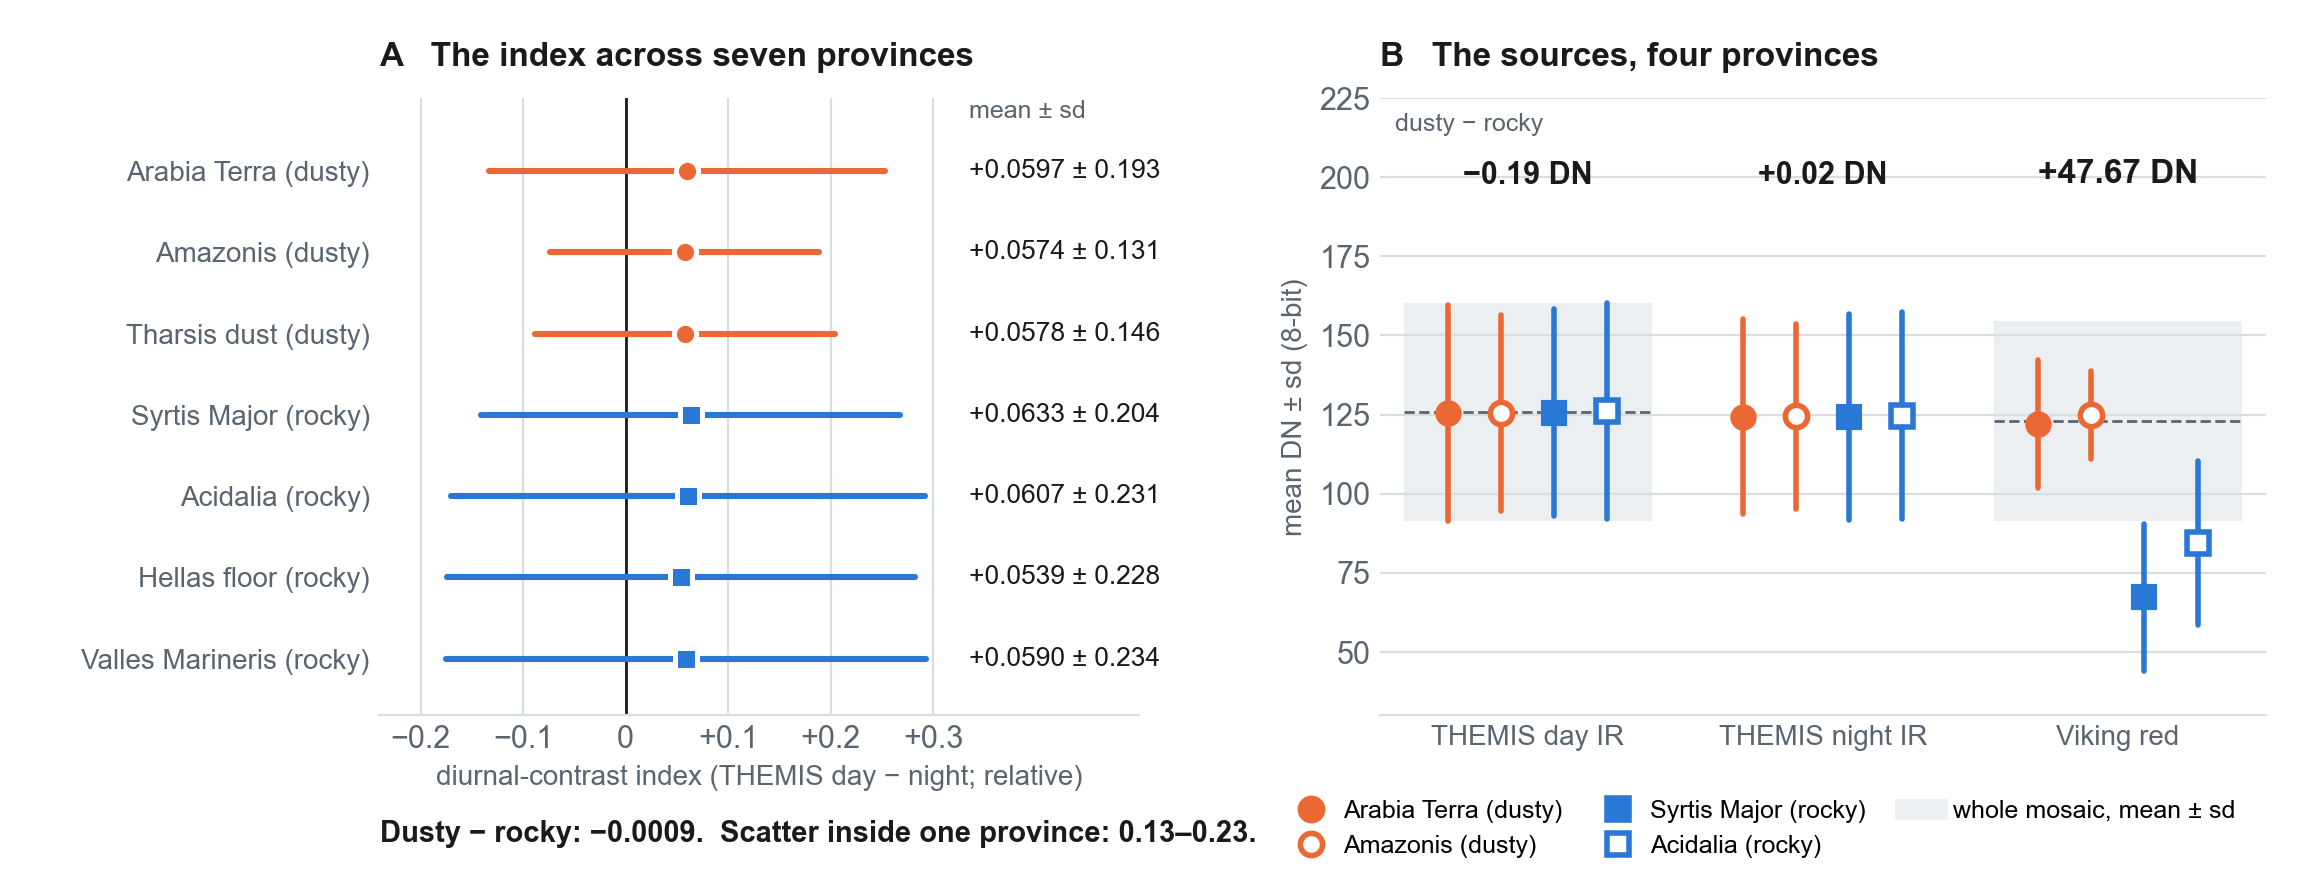
\includegraphics[width=\textwidth]{figures/global60_thermal.png}
\caption{(A) The diurnal-contrast index over seven provinces: dusty and rocky provinces differ by $-0.0009$. (B) The
source DN of four provinces: the THEMIS mosaics repeat the mosaic-wide mean and spread everywhere, while Viking red
keeps a 47.67~DN albedo difference. \label{fig:provinces}}
\end{figure*}

Calibrated inertia agrees (Figure~\ref{fig:tes}). Averaged into TES cells ($\sim3$~km), Viking red tracks log thermal
inertia across \pmsixty\ ($r=-0.31$ dayside, $-0.36$ nightside), much less within a $15^{\circ}$ block (median
$-0.06$, $-0.10$): a regional signal, the dust provinces. Night infrared and the index carry a weak local signal in the
physical direction (median within-block $r=+0.11$ and $-0.08$ against nightside inertia, quartiles of one sign) that
vanishes planet-wide, as region-by-region stretching predicts; day infrared carries none. In the type areas the index
tracks nightside inertia weakly at Ius ($r=-0.22$) and not at all at Athabasca ($-0.01$), where Viking albedo does
($-0.64$). The prediction that the index would track inertia clearly in both windows fails. %% KB §43.1, §42.4

\begin{figure}[t]
\centering
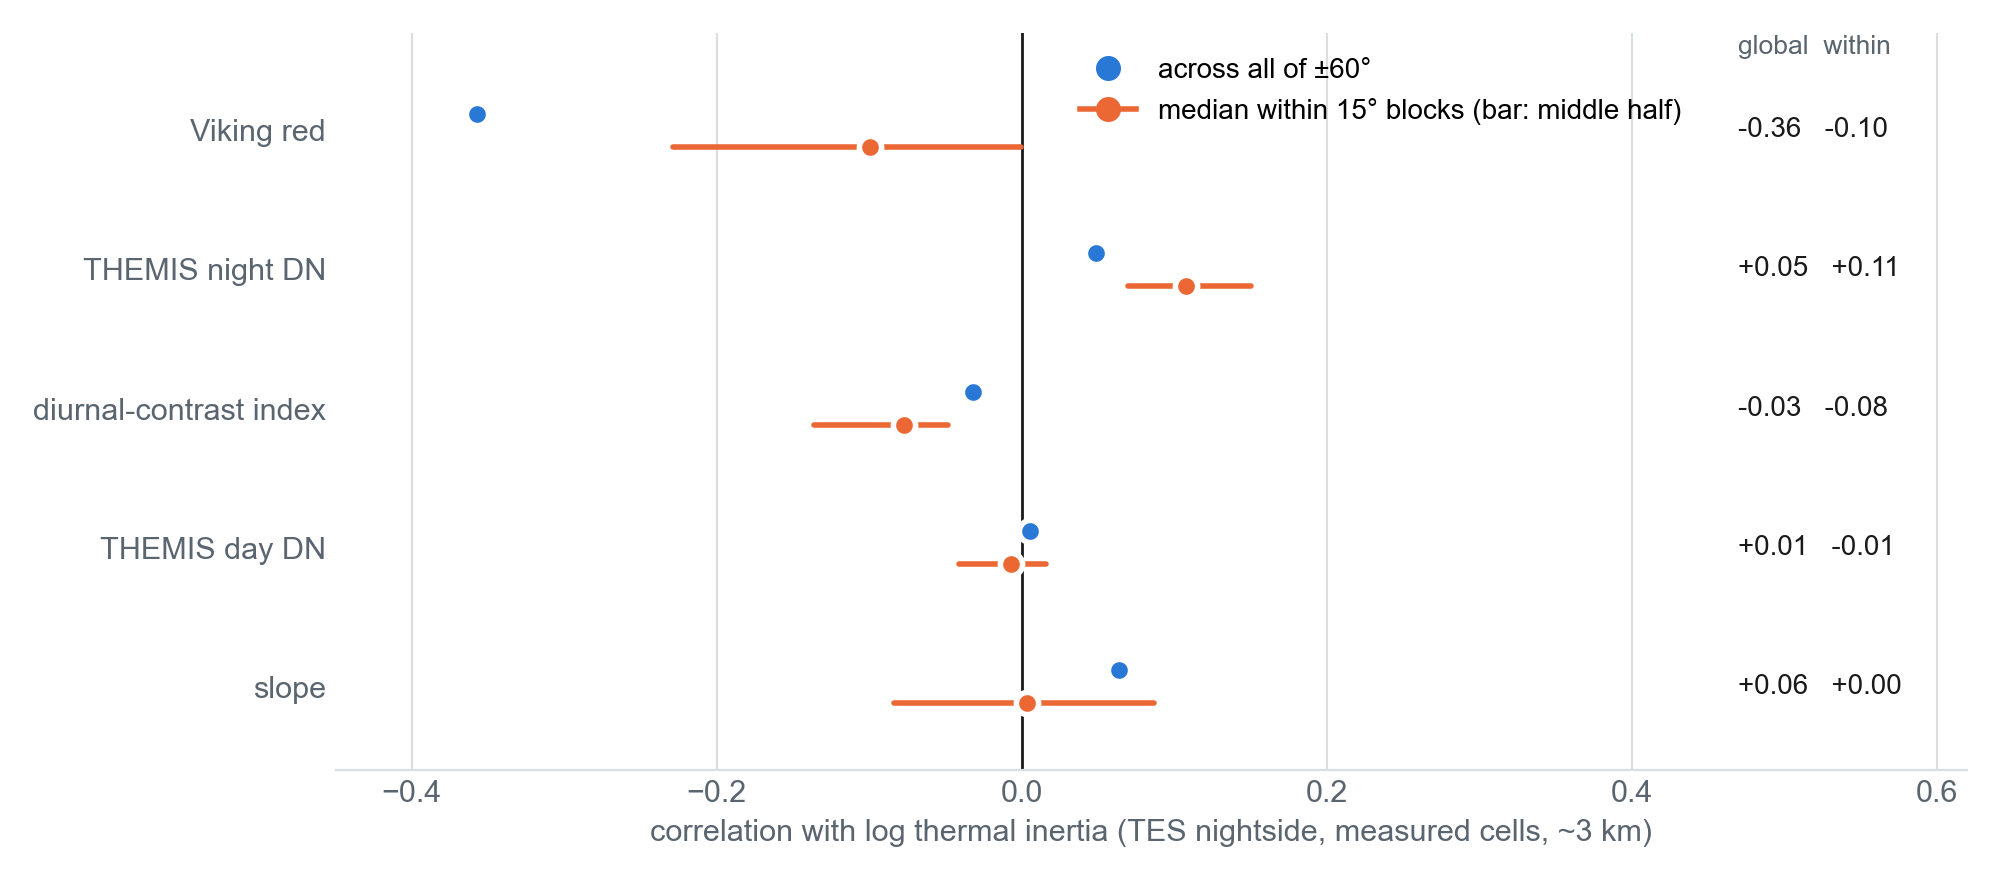
\includegraphics[width=\columnwidth]{figures/tes_check.png}
\caption{Correlation of each \pmsixty\ layer with log TES nightside thermal inertia \citep{Putzig2007} in measured
cells ($\sim3$~km): across the whole extent (blue) and the median within $15^{\circ}$ blocks with its interquartile
range (orange). \label{fig:tes}}
\end{figure}

\subsection{Craters}

The basin pass finds 217,622 closed depressions at 1.6~km in 48~s, 5,144 of them $\ge20$~km, including Hellas
(2,697~km across, 7,857~m deep), Utopia (2,093~km) and Isidis (1,026~km). Of the 117 named IAU craters $\ge100$~km
inside $\pm58^{\circ}$, 88 (75\%) have a closed depression near their centre and 79 (68\%) one whose diameter is within
50\%; on those the median diameter error is $+2.2\%$ (10th and 90th percentiles $-12.6\%$ and $+20.8\%$). This answers
H4 with fill depth rather than image gradients. %% KB §28.11

The fine pass at 200~m, 11~h on the workstation, yields 465,354 closed depressions $\ge1$~km with clean tile seams
(density across seams 0.990 and 0.979 of mid-tile). Against Robbins (Figure~\ref{fig:robbins}), a candidate matches if
its centre lies within half the catalogued diameter and its diameter within a factor of two; a chance baseline shifts
every candidate east by three of its own diameters. Precision rises from 15.3\% at $\ge1$~km to 62.2\% at $\ge5$~km
and 83.1\% at $\ge20$~km, against chance below 11\% at every size; recall levels off near one half, because breached
and degraded craters are not closed. In the type areas the same rule gives a precision of 11\% (Ius) and 13\%
(Athabasca) at $\ge1$~km. %% KB §53.4, §54.4, §42.3; logs\global60_candidates_check.json

\begin{figure*}[t]
\centering
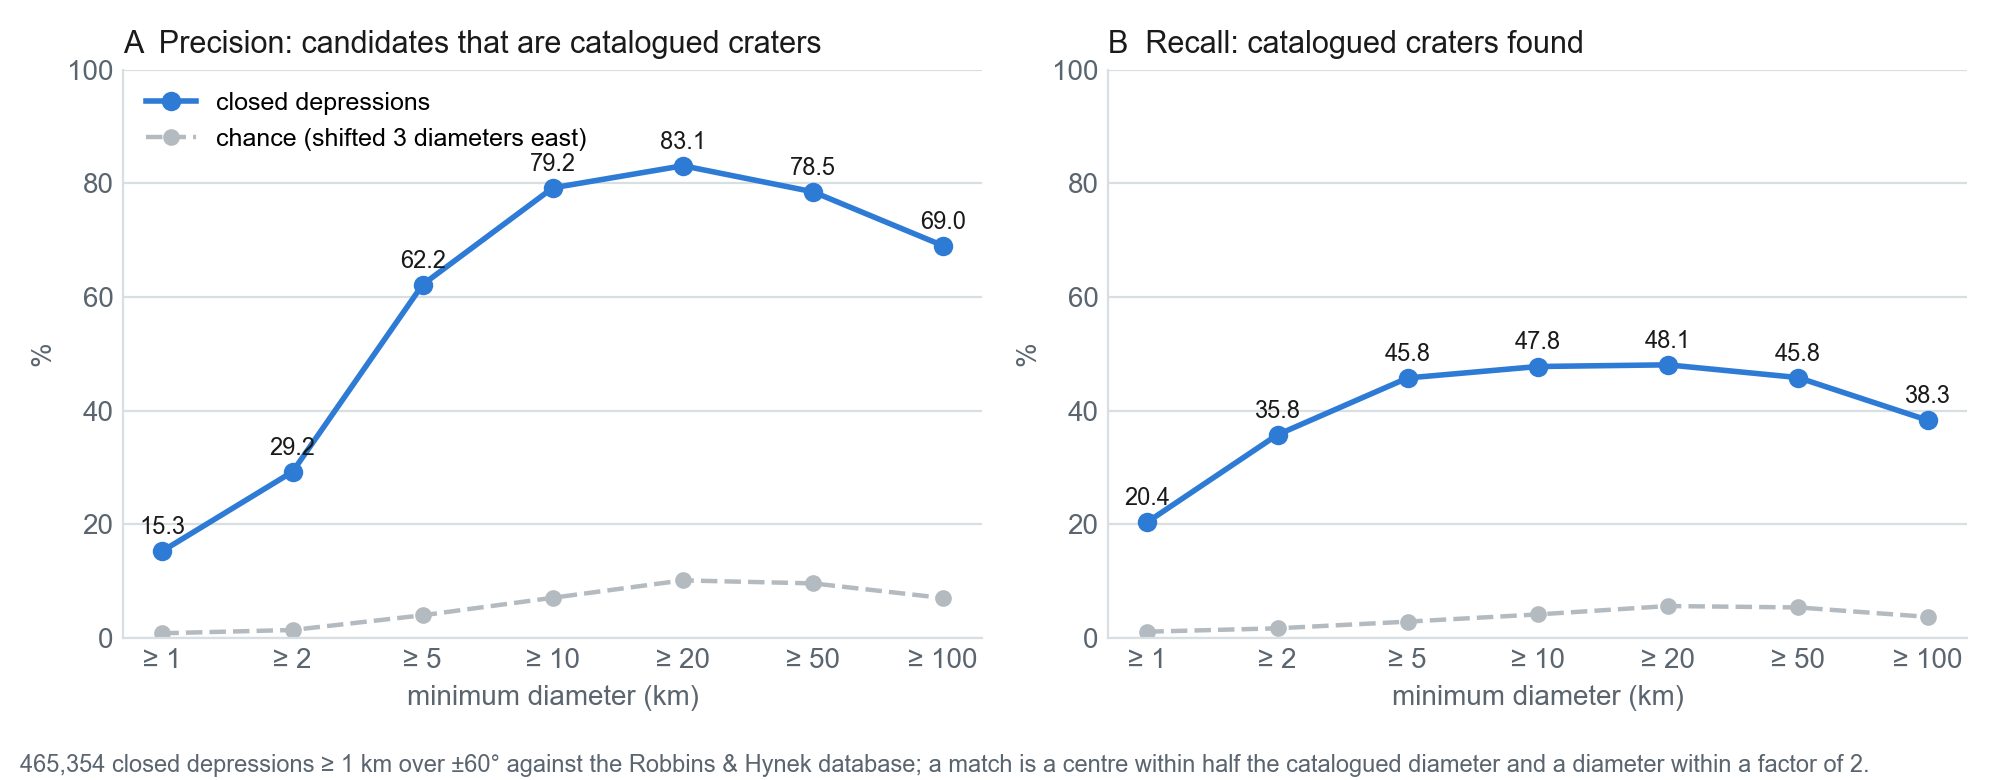
\includegraphics[width=\textwidth]{figures/depressions_vs_robbins.png}
\caption{The 465,354 closed depressions $\ge1$~km against the Robbins and Hynek crater database
\citep{Robbins2012} by minimum diameter: (A) precision, (B) recall, each beside a chance baseline made by shifting
every candidate three of its diameters east. \label{fig:robbins}}
\end{figure*}

Mapped by density, the small candidates do not follow the craters: per 0.5$^{\circ}$ cell their log density correlates
with that of Robbins at $r=-0.11$, nearly flat across latitude bands while Robbins doubles, and their pattern shows
north--south stripes where the HRSC/MOLA blend is sharpest. Below about 5~km the detector maps the elevation model's
resolution as much as the craters. Relative crater density per geologic unit, which needs no detector, ranks the units
as expected: on \lAv\ Robbins counts 1,122 craters $\ge1$~km per $10^6$~km$^2$, against 1,760 and 2,183 on the older
units of the Athabasca window; the detector reverses the order (4,966 on \lAv) by counting non-crater pits on flat lava.
These densities are relative and are not converted to ages \citep{Hartmann2005}. %% KB §53.6, §42.2

\subsection{Channels}

At Ius Chasma, \texttt{Fill} raised 21.7\% of the scene by more than 1~m and the canyon floor by up to 2,077~m, and
56.1\% of the first routed network ran across that synthetic surface (Figure~\ref{fig:fill}). It looked plausible:
long, smooth, dendritic trunks down the chasma. With the fill mask, 2,610 candidates (15,428~km) remain; 64\% lie on
plateau under $2^{\circ}$ where routing follows noise, and 188 are steep ($\ge5^{\circ}$) and rock-floored (index
$<-0.15$), the subset worth review. %% KB §25.1, §25.2

\begin{figure}[t]
\centering
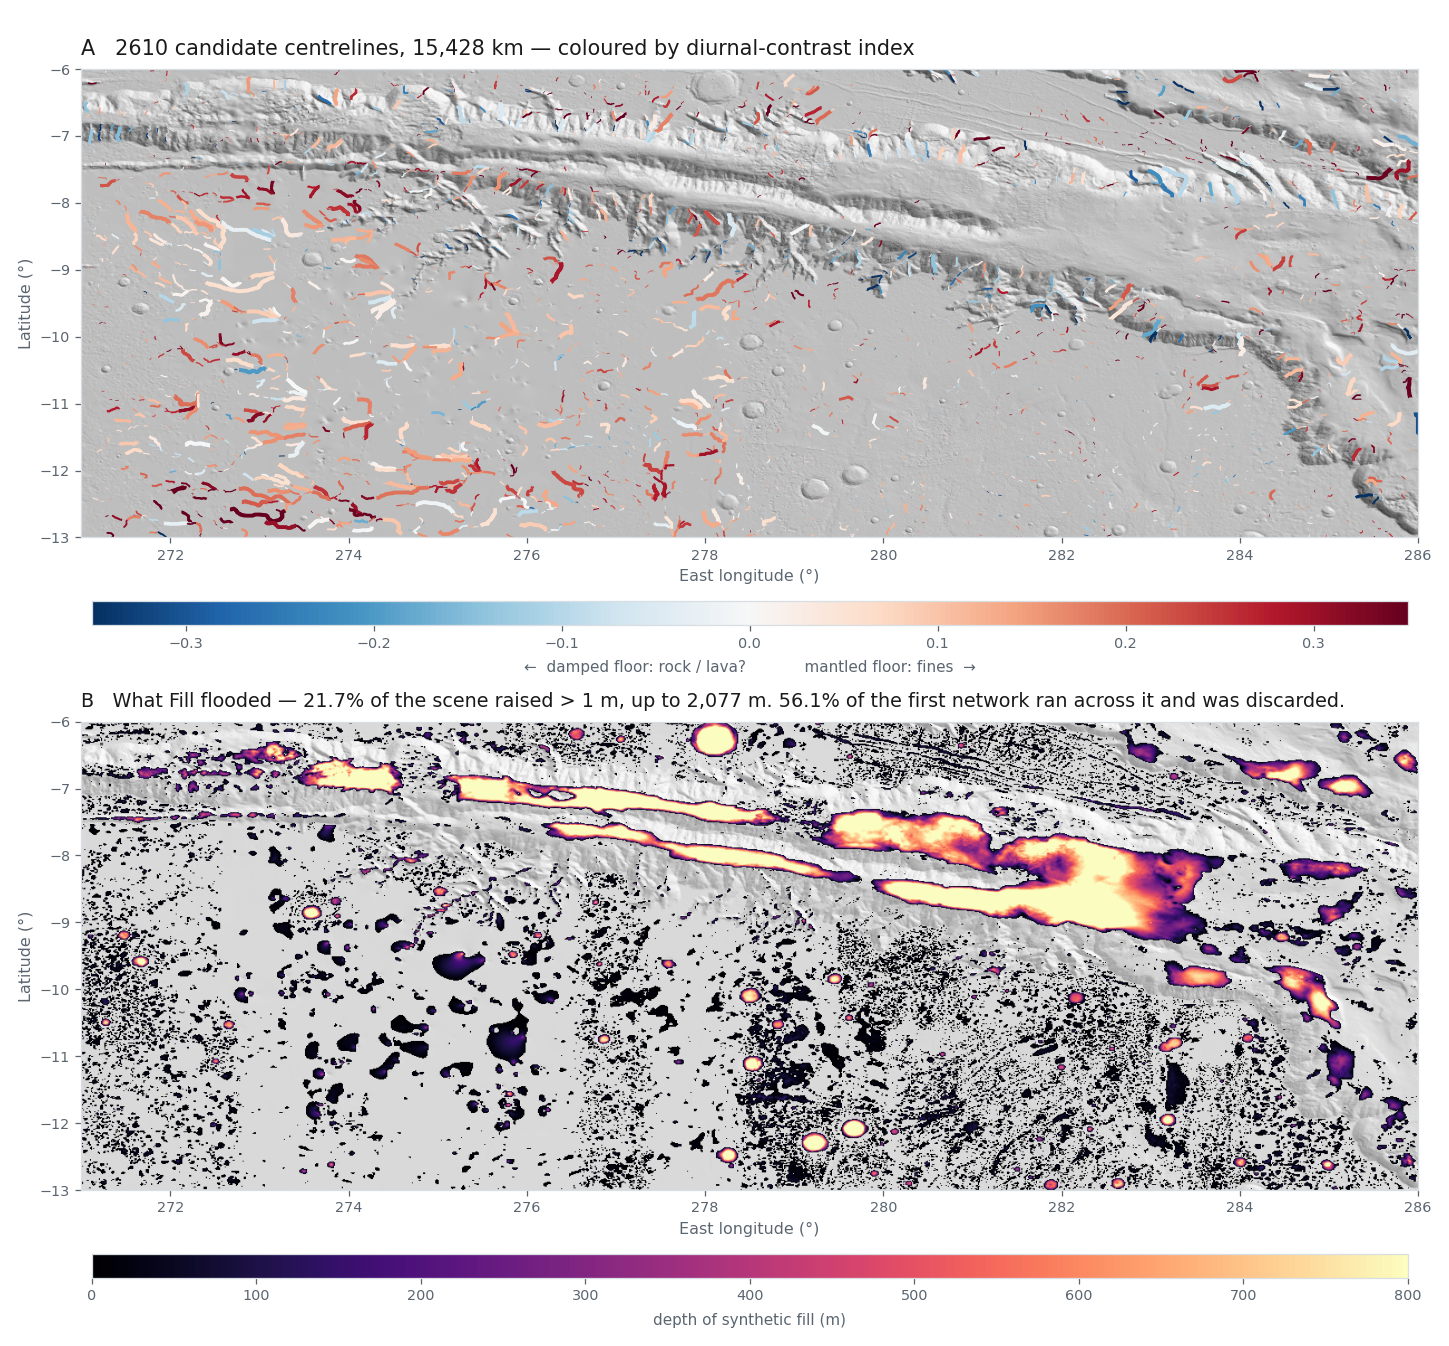
\includegraphics[width=\columnwidth]{figures/ius_channel_candidates.png}
\caption{Channel candidates at Ius Chasma. (A) The 2,610 centrelines kept after the fill mask, coloured by the
diurnal-contrast index. (B) Where \texttt{Fill} flooded the surface: 21.7\% of the scene raised by more than 1~m, up to
2,077~m; 56.1\% of the first network ran across it and was discarded. \label{fig:fill}}
\end{figure}

At \pmsixty\ the fill mask discards 60.5\% of stream cells and leaves 969,822 segments (6.17 million km;
orders 1--5: 564,882, 360,236, 41,442, 3,165 and 97; Figure~\ref{fig:channels}). Of 40,410 sampled midpoints, 89.8\%
lie on ground under $2^{\circ}$, and 96.7\% of those of order 3 and higher: the long high-order paths gather on smooth
ground where the DEM holds few pits, and their length per cell correlates negatively with the density of 1--2~km
depressions ($r=-0.35$). The network is not scored here; the global valley maps of \citet{Hynek2010} and
\citet{Alemanno2018} are the natural references, and the second is held for that test. %% KB §54.4, §55.4, §53.6, §68.5; NEXT-STEPS §12.2 A1

\begin{figure*}[t]
\centering
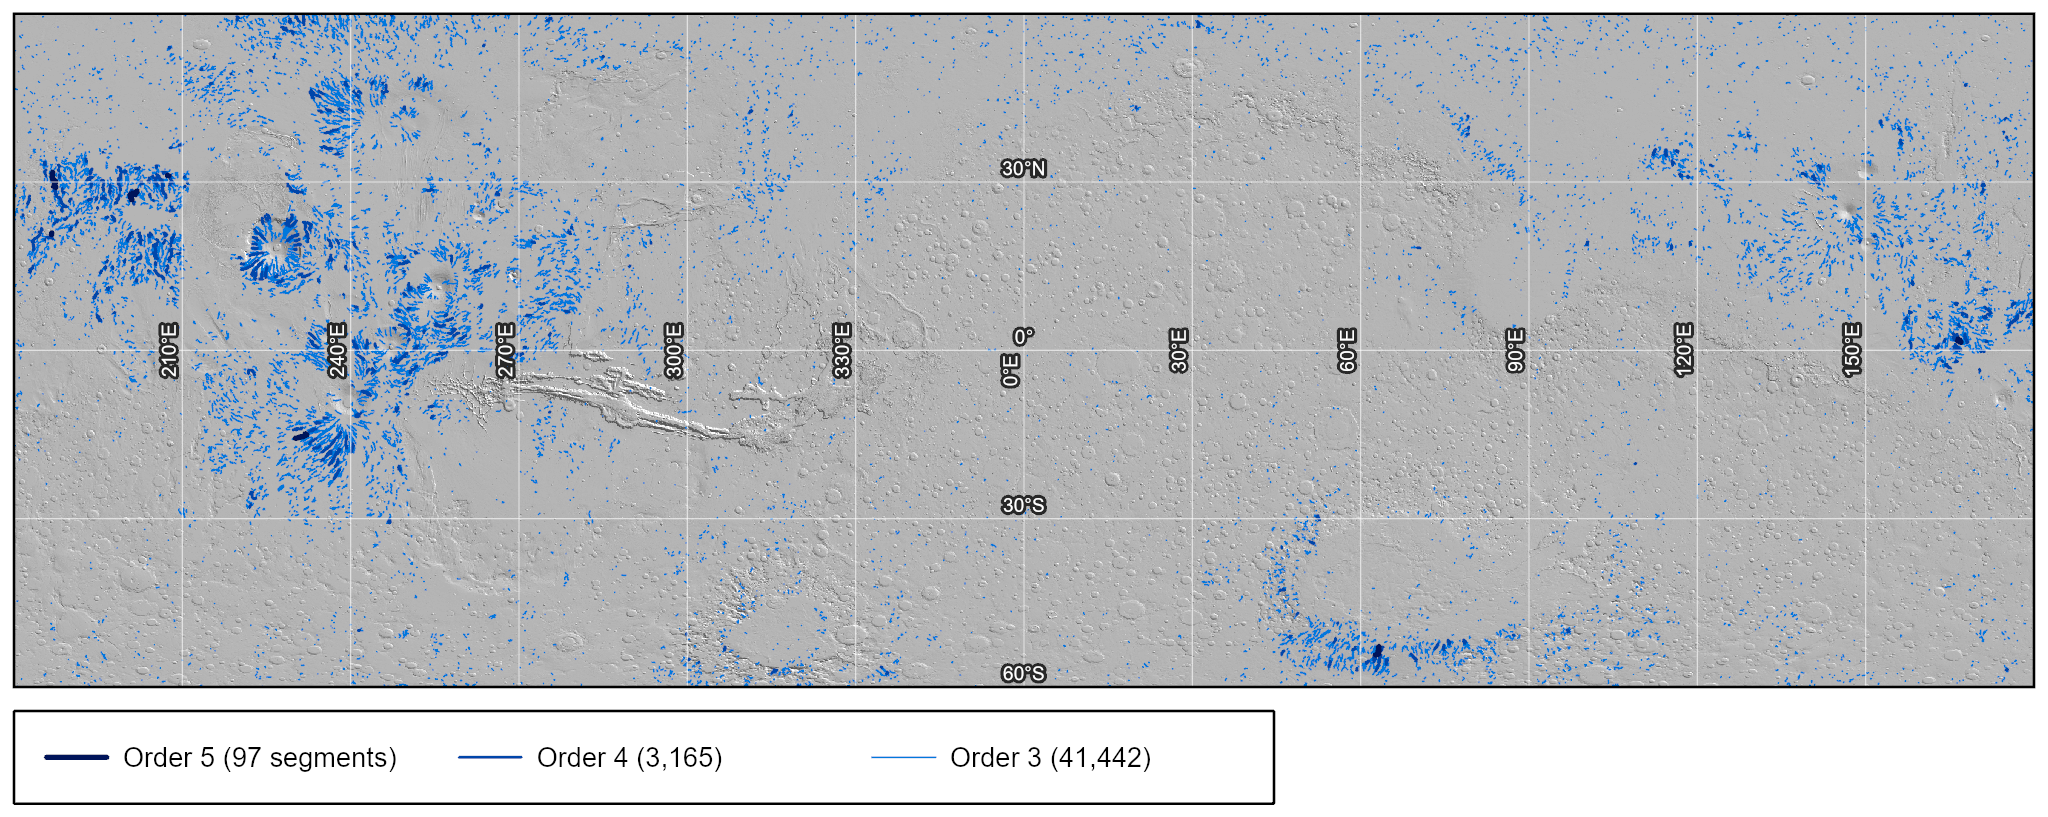
\includegraphics[width=\textwidth]{figures/12_global60_channels.png}
\caption{Routed channels of Strahler order 3 to 5 over the \pmsixty\ hillshade (orders 1 and 2 are not drawn). Most
high-order paths lie on plains under $2^{\circ}$ and follow the DEM's makeup as much as real drainage. \label{fig:channels}}
\end{figure*}

How many tributary orders the 100~m stack resolves (test T7) has no answer the elevation model supports. Over
thresholds from 1 to 500~km$^2$ at Ius Chasma, the highest order falls from 5 to 2, about one order per tenfold rise in
the threshold, while only 30.8--36.7\% of first-order cells lie on slopes $\ge2^{\circ}$ (53.3\% of the window does); the
rule set in advance (first-order streams at least half on $\ge2^{\circ}$) is met by no threshold. %% KB §47.4

H2 was tested at a first stage with the window standing in for origin (Ius fluvial, Athabasca volcanic). The volcanic
window's 3,272 candidates are shallower, not steeper, than Ius's 2,588 (median 1.4 against 10.2~m~km$^{-1}$, difference
$-8.85$~m~km$^{-1}$, interval $-15.69$ to $-5.76$), and the thermal z-score separates the two no better than chance (AUC
0.50, against 0.81 for gradient). What separates them is the setting, chasma walls against lava plains, so stage one
cannot settle H2; stage two waits for reviewed channels with their origin set. %% KB §51.1

\subsection{Lava flows}

The classification's lava-tube class does not find lava plains. Against SIM~3292 unit groups, expressed as enrichment
$P(\mathrm{class}\mid\mathrm{group})/P(\mathrm{class})$ (Figure~\ref{fig:t8}), lava tube is slightly depleted on volcanic
plains ($\times0.84$) and enriched on volcanic edifices ($\times3.30$) and aprons ($\times4.29$): steep volcano flanks.
Normal Ground covers 76\% of the volcanic plains. The other classes sit where the geologic map says they should, so the
map is coherent as a terrain map but is not a lava-flow map. A relabelled class trained on the map's volcanic units
fared worse: as a fifth class it lowered the other three classes' held-out accuracy from 70.2\% to 64.6\%, and only 30\%
of what it called volcanic was, below the 38\% base rate. Lava flows in this study therefore come from the geologic
map's volcanic units. %% KB §43.2, §43.3, §57.1

\begin{figure*}[t]
\centering
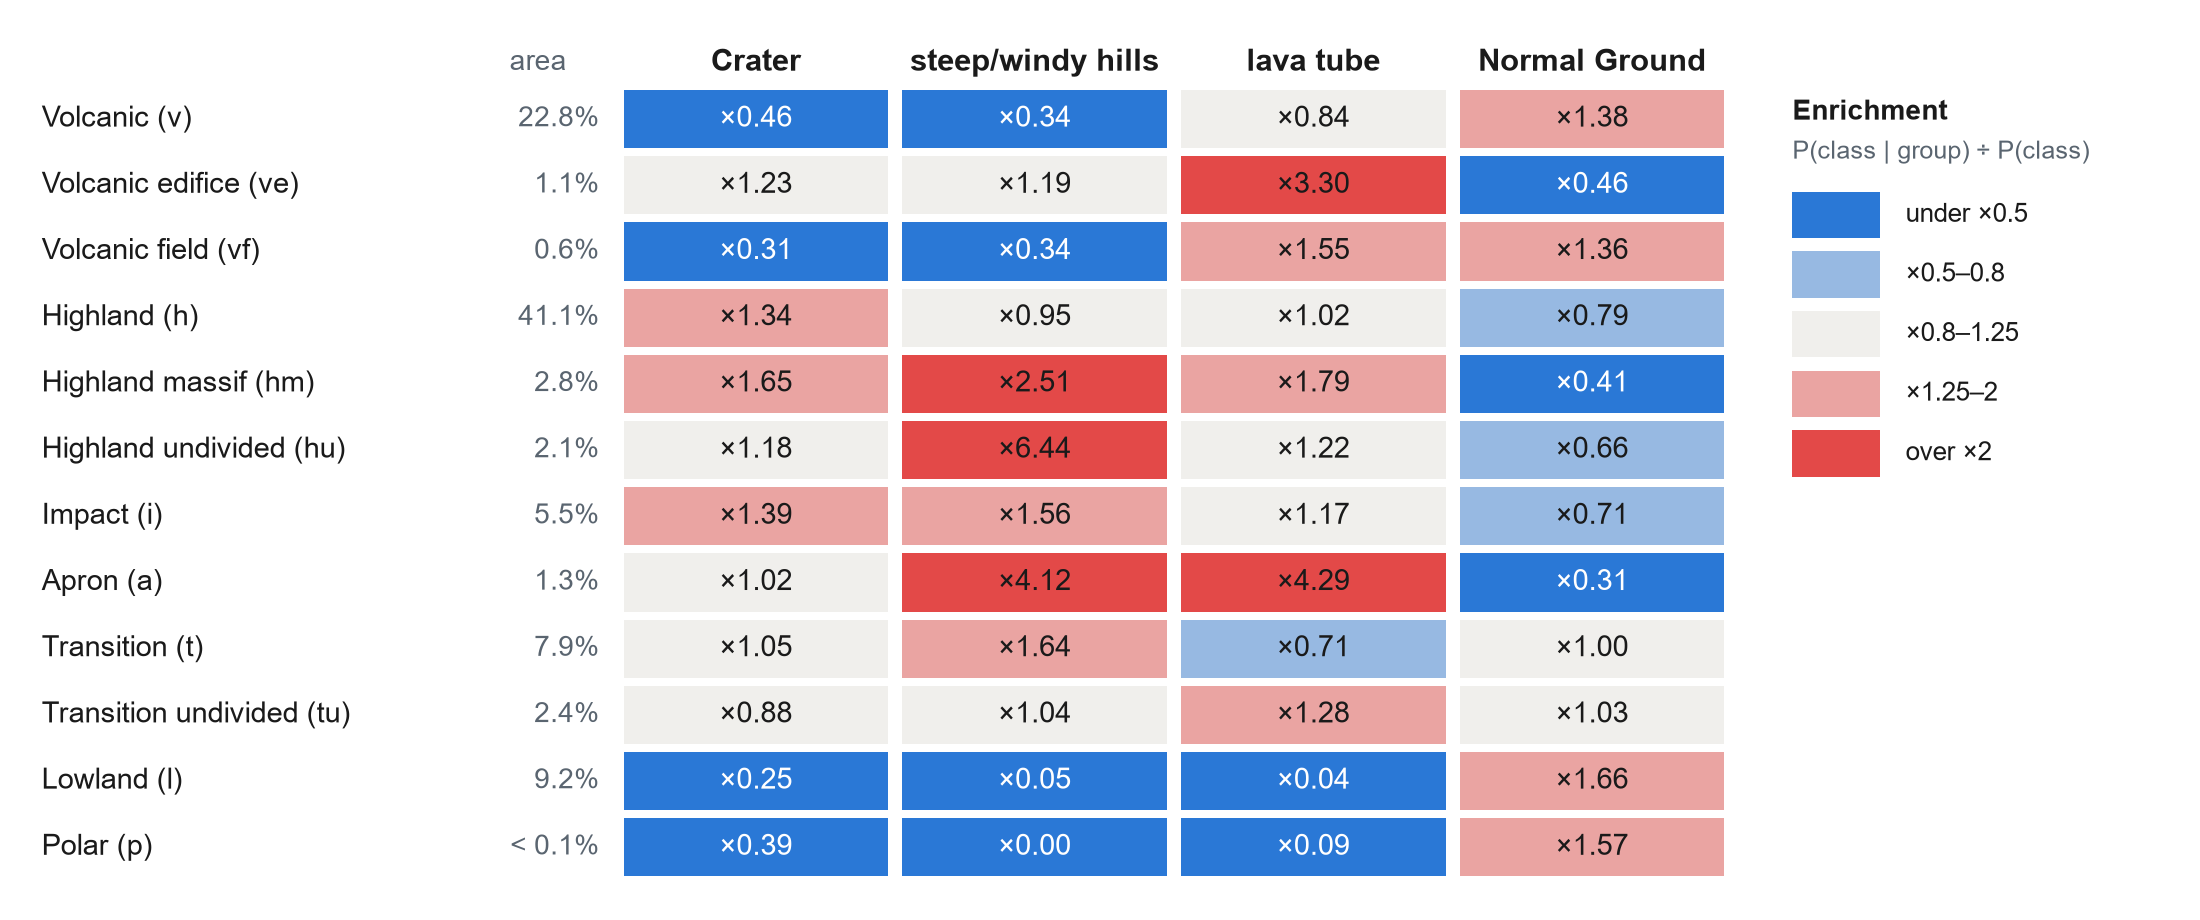
\includegraphics[width=0.85\textwidth]{figures/t8_enrichment.png}
\caption{The published landform map against the unit groups of SIM~3292: how much more often each class occurs in a
group than across \pmsixty\ ($\times1$: no association). \label{fig:t8}}
\end{figure*}

H1 was tested on the 14 internal contacts (2,764~km) between the five SIM~3292 units of the Athabasca window. Profiles
every 2~km, $\pm20$~km perpendicular to each contact, count as separating when the contrast across them exceeds the 90th
percentile of 2,000 random profiles, so chance is 10\% (Figure~\ref{fig:t5}). Across the 905 profiles on the ten
contacts of \lAv, day infrared separates 21.0\% (interval 3.3--38.4\%), Viking red 12.3\%, night infrared 11.7\% and
the index 13.0\%. Day infrared leans toward H1 by $+8.7$ points over Viking red, but the interval ($-1.7$ to $+18.1$)
includes zero, so by the rule set in advance H1 is not supported. A map at 1:20\,M generalises contacts by kilometres,
and ten contacts cannot settle the question; H1 needs margins digitised on the 100~m stack. %% KB §47.2

\begin{figure*}[t]
\centering
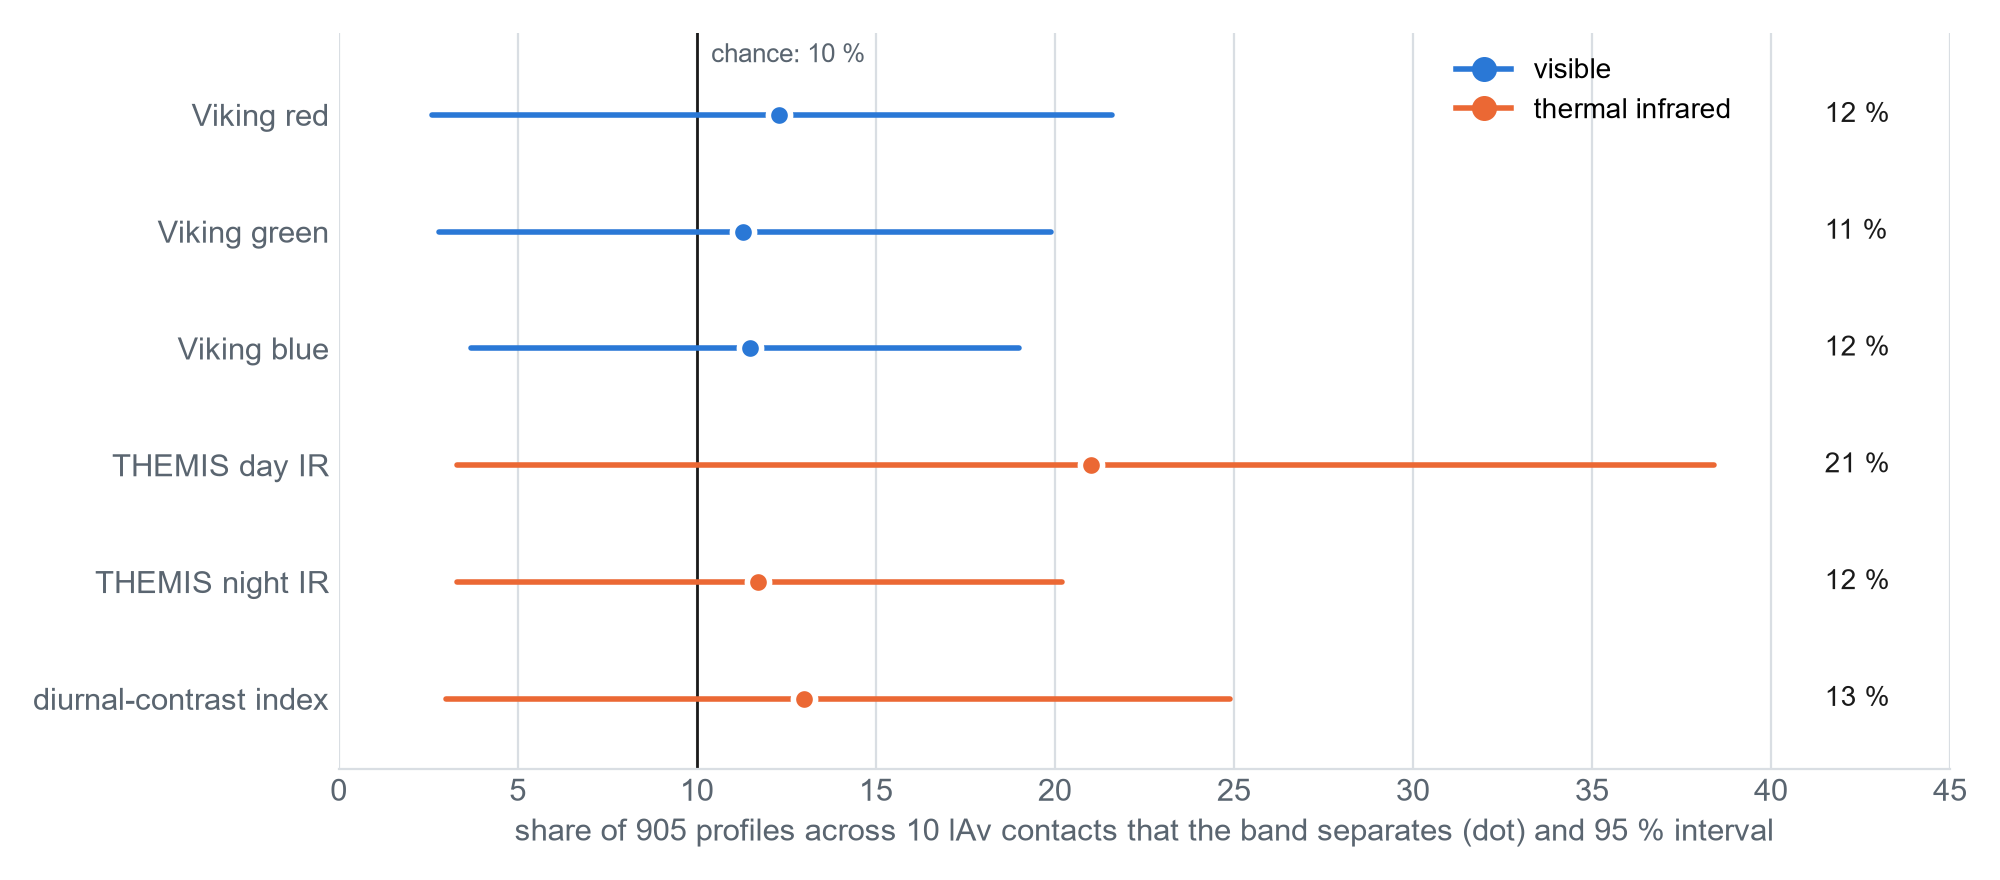
\includegraphics[width=0.75\textwidth]{figures/t5_margins.png}
\caption{Test T5 (H1): the share of profiles across the geologic map's contacts at Athabasca Valles that each band
separates, with bootstrap intervals over contacts; 10\% is chance by construction. \label{fig:t5}}
\end{figure*}

\subsection{The landform classification}

The published map (Figure~\ref{fig:landforms}) is the 200~m support vector machine map with an $11\times11$ (2.2~km)
majority filter. On the 183 held-out polygons it scores 73.8\%, \kap\,0.583, against 58.6\% for one class everywhere and
69.9\%, \kap\,0.532 unfiltered (Table~\ref{tab:svm}, Figure~\ref{fig:accuracy}). Normal Ground is found almost
everywhere it was drawn (producer's 99.2\%) and Crater is reliable where mapped (user's 93.3\%), but lava tube is not a
usable class (user's 2.4\%). Halving the cell from 400~m bought no held-out accuracy (70.5\% raw at 400~m). The map is
no longer an elevation map (elevation bins reproduce 55.4\%, within a point of its largest class alone, 54.7\%), shows
no tile seams (ratio 1.00), and labels 56.8\% of the ground inside named craters as Crater against 46.2\% in the ring
around them. %% KB §55.3, §57; logs\global60_classification_check_200m_mode11.json

The overall score flatters the map. Crater is 58.6\% of the held-out area, and its balanced accuracy is 66.7\% with a
mean F1 of 55.7\%, lava tube's F1 being 4.5\%. Of the 26.2 points of disagreement, 20.5 are quantity and 5.7
allocation: most of the error is in how much of each class the map paints, not where, giving 38.1\% of the held-out
ground to Crater against the labels' 58.6\% and painting the rest of the Crater polygons lava tube (10.9 points),
Normal Ground (8.1) and hills (4.1). Over all of \pmsixty\ it is 54.7\% Normal Ground, 33.9\% Crater, 9.4\% lava tube
and 1.9\% hills. %% KB §69.18; logs\score_metrics.json

\begin{figure*}[t]
\centering
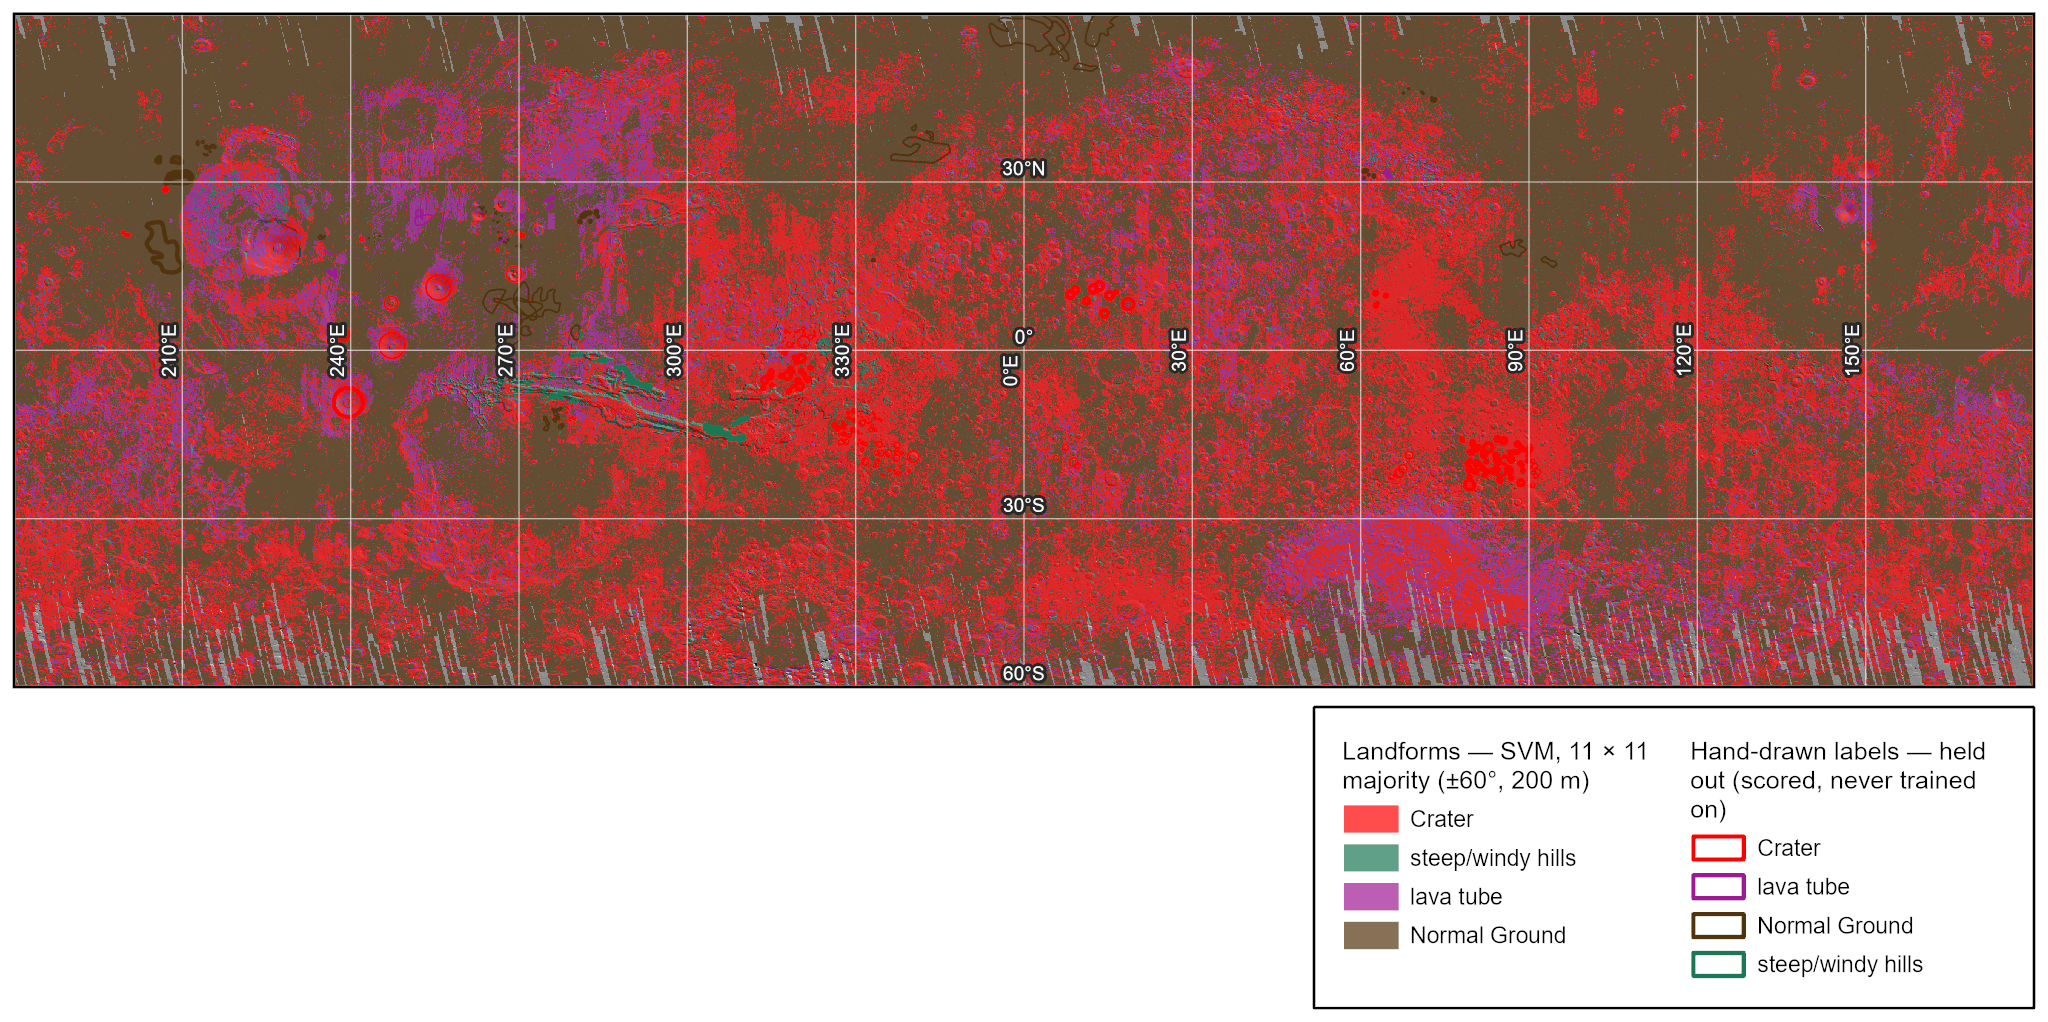
\includegraphics[width=\textwidth]{figures/04_global60_landforms.png}
\caption{The published \pmsixty\ landform map: support vector machine on the seven-band 200~m stack, $11\times11$
majority filter, with the held-out hand-drawn labels outlined in their class colours. Held out: 73.8\%, \kap\,0.58.
\label{fig:landforms}}
\end{figure*}

\begin{figure*}[t]
\centering
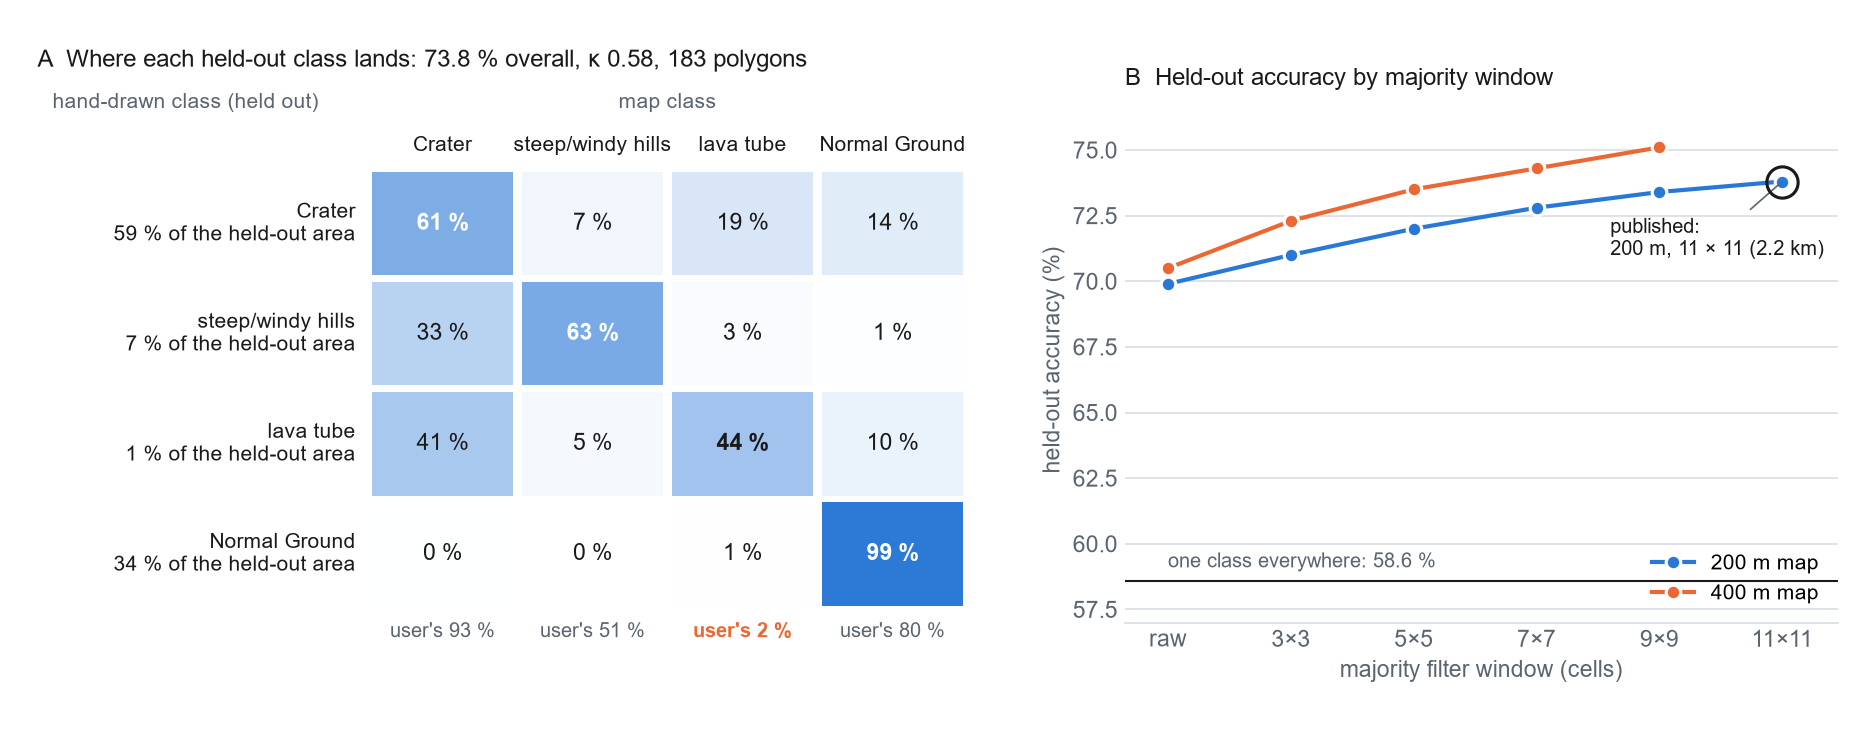
\includegraphics[width=\textwidth]{figures/accuracy_200m.png}
\caption{(A) Where each held-out class lands on the published map, as a share of its area. (B) Held-out accuracy
against the majority-filter window for the 200~m and 400~m maps; the score rises with every window, so the window was set
by feature size. \label{fig:accuracy}}
\end{figure*}

\begin{table}[t]
\centering
\caption{Held-out scores of the landform maps (183 polygons) \label{tab:svm}}
\small
\setlength{\tabcolsep}{3.5pt}
\begin{tabular}{lcccccc}
\hline\hline
Map & Acc. & $\kappa$ & Bal. & F1 & Q & A \\
\hline
One class everywhere & 58.6 & -- & -- & -- & -- & -- \\
SVM 400 m, raw & 70.5 & 0.540 & 63.5 & 53.4 & 23.6 & 5.9 \\
SVM 200 m, raw & 69.9 & 0.532 & 63.1 & 52.8 & 24.2 & 5.9 \\
SVM 200 m, $5\times5$ & 72.0 & 0.560 & 65.1 & 54.4 & 22.2 & 5.8 \\
SVM 200 m, $11\times11$$^{a}$ & 73.8 & 0.583 & 66.7 & 55.7 & 20.5 & 5.7 \\
U-Net, two passes & 98.9 & 0.980 & 94.8 & 93.9 & 0.5 & 0.6 \\
\hline
\end{tabular}
\par\vspace{3pt}\noindent\parbox{\columnwidth}{\footnotesize Note: In percent but $\kappa$. Acc., overall accuracy;
Bal., balanced accuracy; F1, mean per-class F1; Q and A, quantity and allocation disagreement ($\mathrm{Q}+\mathrm{A}=
100-\mathrm{Acc.}$). Area-weighted by $\cos$ latitude, scored at 400~m. $^{a}$The published map.}
\end{table}
%% KB §55.3, §57, §66.8, §69.18

Whether the thermal bands help (test T1) was measured twice, with the prediction of little or no gain written first.
A Gaussian maximum-likelihood ablation on 2.69 million held-out pixels (Figure~\ref{fig:ablation}) finds that the
thermal bands add $+1.3$ points (interval $+0.6$ to $+2.2$), that slope and relief alone (68.6\%) match all seven bands
(67.0\%), and that without terrain the visible and thermal bands score below the one-class baseline (42.4\%).
Retraining ArcGIS Pro's support vector machine over all of \pmsixty\ without each band group confirms it
(Table~\ref{tab:t1}): the thermal gain is the one difference resolved at both cells. It is not uniform: thermal helps
Crater (producer's $+1.9$ points, nine more polygons won) and hills ($+5.5$ points) and hurts lava tube ($-8.5$
points). Weighted by class rather than by area, the gain disappears: balanced accuracy is 63.1\% with the thermal
bands and 63.4\% without at 200~m, 63.5\% and 63.4\% at 400~m, because Crater and hills hold most of the held-out
area. Terrain alone ties the score but makes a poor crater map (34 of 124 crater polygons won, against 103). The
hand-drawn classes are landform classes, a terrain property, and cannot price a material signal. %% KB §40.1, §56, §56.1, §69.18

\begin{figure}[t]
\centering
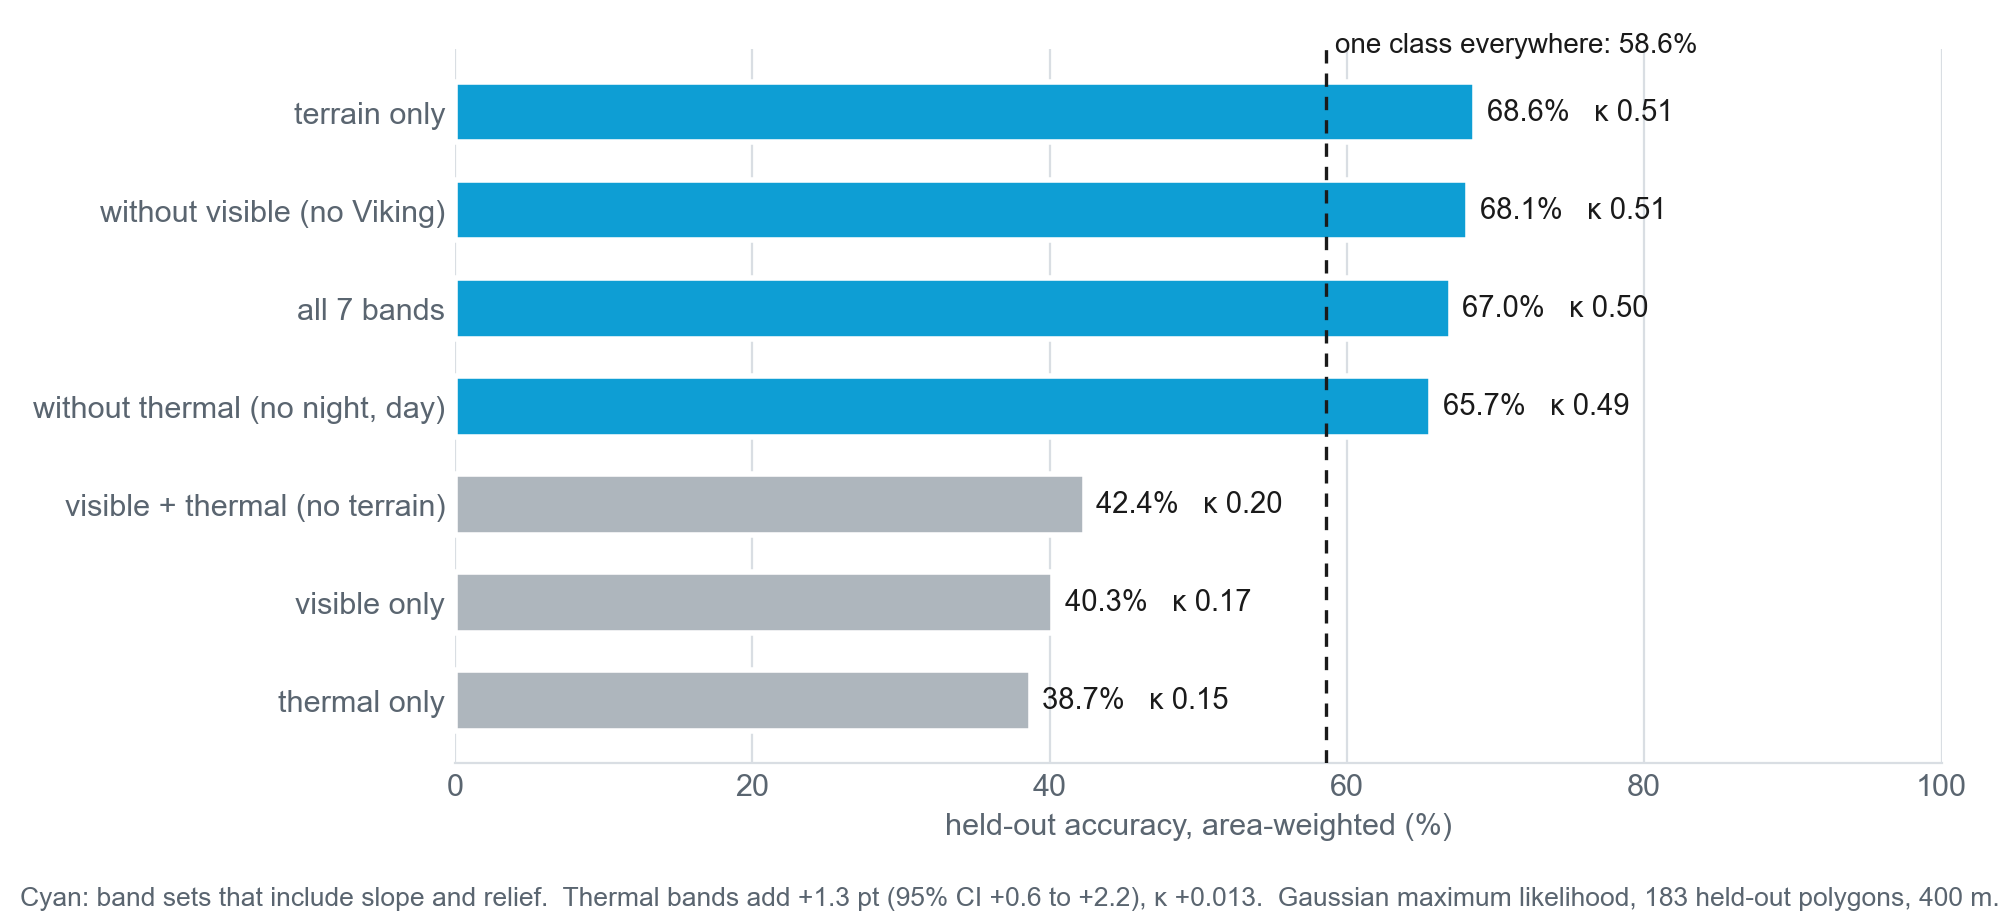
\includegraphics[width=\columnwidth]{figures/thermal_ablation.png}
\caption{Test T1, first form: held-out accuracy of a Gaussian maximum-likelihood classifier on each band set at 400~m.
The dashed line is one class everywhere. \label{fig:ablation}}
\end{figure}

\begin{table}[t]
\centering
\caption{Test T1 with ArcGIS Pro's support vector machine \label{tab:t1}}
\small
\begin{tabular}{llcc}
\hline\hline
Cell & Left out & Gain (pt) & 95\% interval \\
\hline
200 m & thermal & $+1.36$ & $+0.46$, $+2.47$ \\
400 m & thermal & $+1.97$ & $+1.08$, $+3.35$ \\
400 m & visible & $-4.26$ & $-10.96$, $+2.18$ \\
400 m & visible and thermal & $-0.30$ & $-6.54$, $+7.73$ \\
\hline
\end{tabular}
\par\vspace{3pt}\noindent\parbox{\columnwidth}{\footnotesize Note: Gain is the held-out accuracy of the all-band map minus that of the map without the group; paired bootstrap over 183 polygons, 1,000 resamples.}
\end{table}
%% KB §56.1

\subsection{Deep learning}

The RetinaNet detector found 41.9\% of held-out Crater polygons with 87.6\% of its in-polygon boxes correct (always
naming Crater gives 71.1\%) and 22.7\% of Normal Ground polygons at 56.9\% precision, but never named hills or lava
tube (Figure~\ref{fig:dl}, left). Retrained with the backbone unfrozen for 30 epochs and with extra chips of the rare
classes, it named hills (25.0\% recall, 100\% precision) but lost Normal Ground (4.5\% recall) and over-predicted lava
tube on craters; by the rule written before the run it did not improve. Boxes suit compact objects \citep{Lee2019}
rather than area classes, and the whole-chip boxes of plains limit this model. %% KB §66.2, §66.5

The U-Net is a different matter. In the held-out windows it scored 98.75\%, \kap\,0.977, and over all of \pmsixty\
98.8\%, but with seams at its 256-pixel tiles (phase ratio 8.6--9.2 against about 1.0 for the support vector machine
maps). The second, offset pass lowered the ratio to 1.2 and changed nothing else measured: 98.9\%, \kap\,0.980 held out,
with lava tube at 77.1\% user's accuracy against 2.4\% (Figure~\ref{fig:dl}, right, and Figure~\ref{fig:unet}). The map
is a map of terrain provinces, not of features: the southern highlands are Crater, the northern lowlands Normal Ground,
lava tube lies on Tharsis and Elysium and hills along Valles Marineris; it makes 55.1\% of \pmsixty\ Crater and
39.3\% Normal Ground, where the support vector machine map makes 33.9\% and 54.7\%. It labels 91.3\% of the ground inside named
craters as Crater, but also 82.6\% of the ring around them, and elevation bins reproduce 68.0\% of it. The held-out
labels mark areas that are mostly one class at 50~km, and a model that sees 51~km of context reproduces those areas; the
score measures agreement with the hand-drawn areas at province scale. The support vector machine map therefore remains
the published landform map, with the U-Net map beside it as a province map. %% KB §66.6, §66.7, §66.8, §66.9

\begin{figure*}[t]
\centering
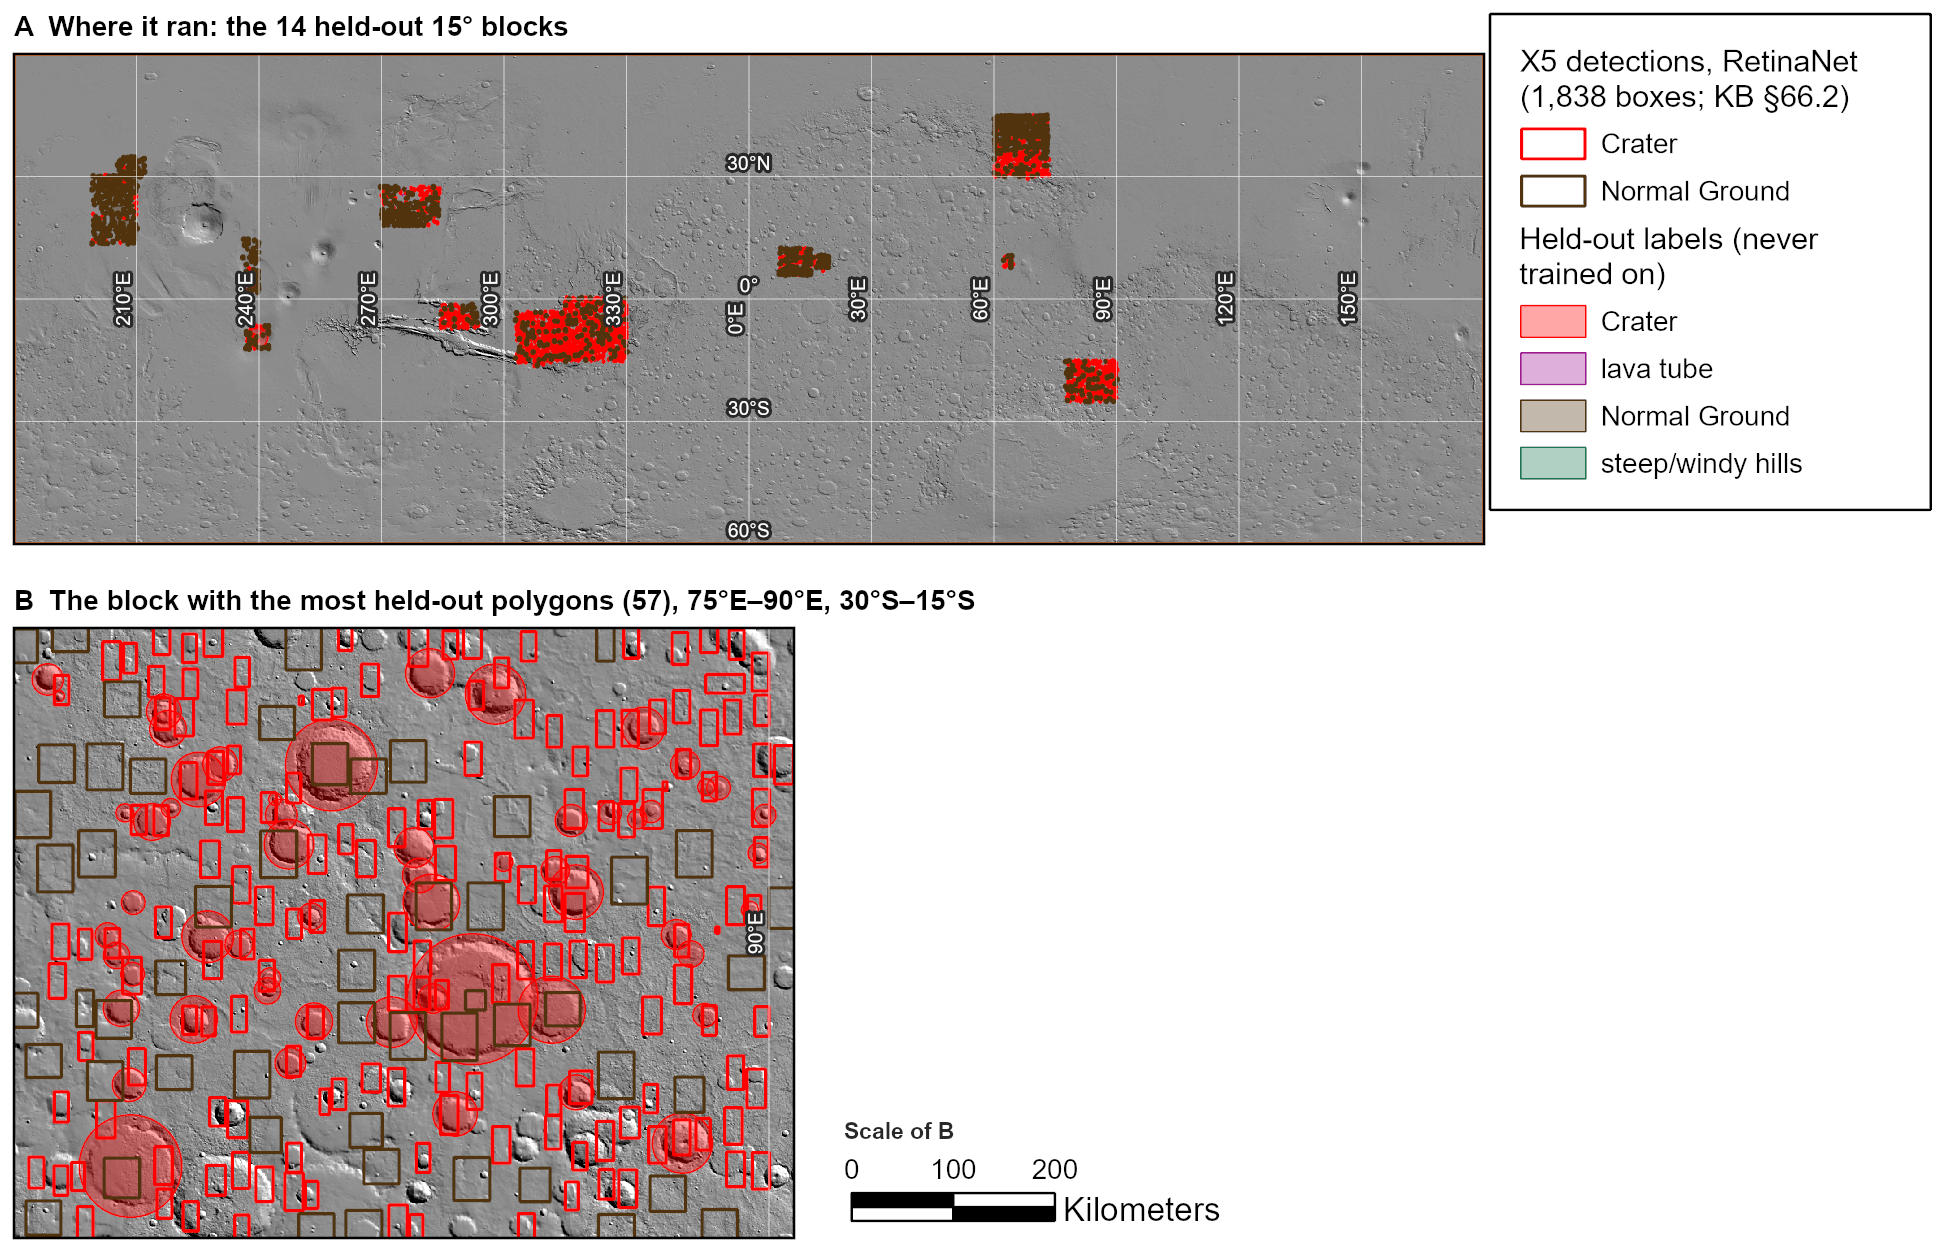
\includegraphics[width=0.49\textwidth]{figures/16_x5_detections.png}\hfill
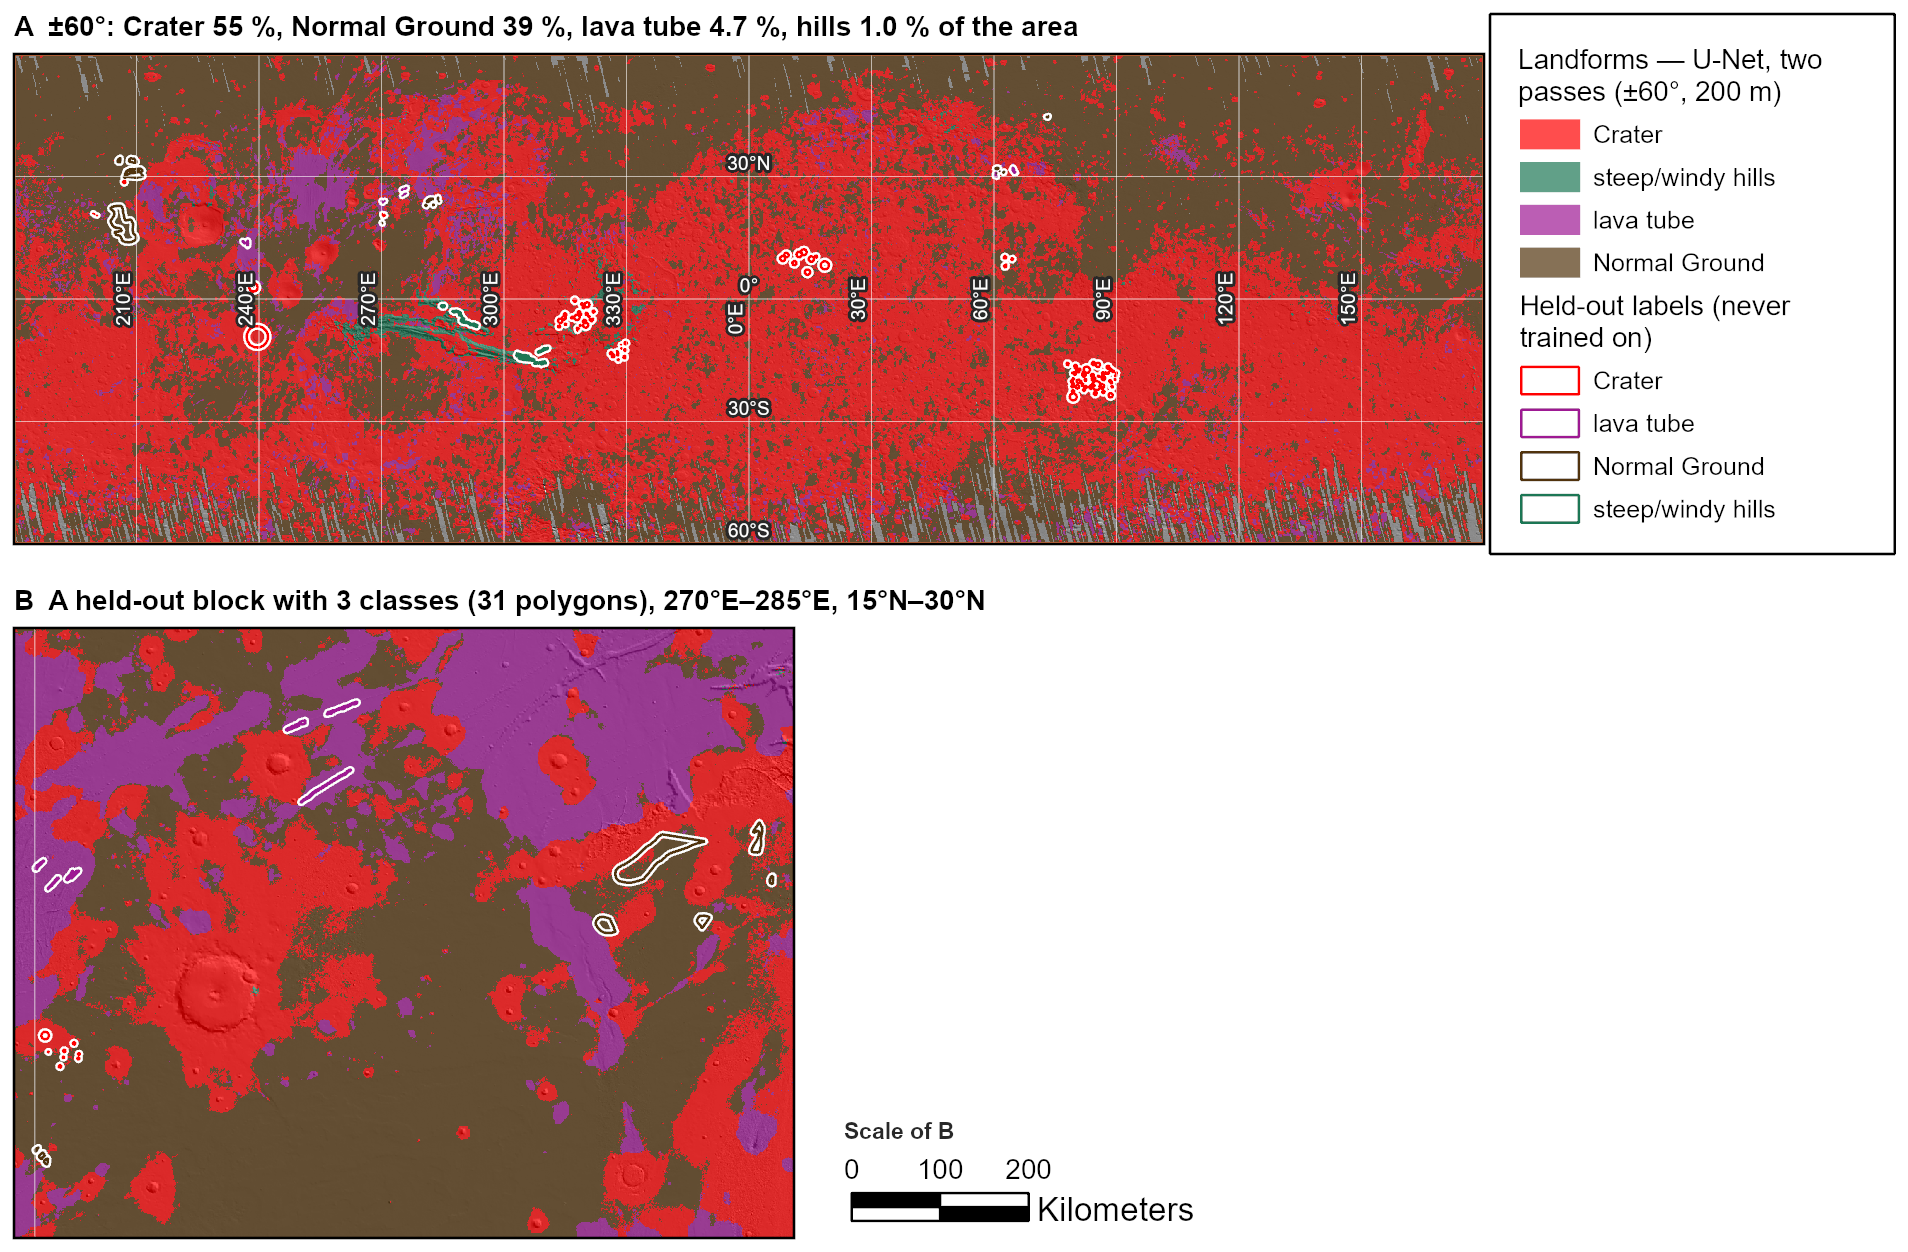
\includegraphics[width=0.49\textwidth]{figures/17_x5c_unet_provinces.png}
\caption{Left: RetinaNet detections in the 14 held-out windows, with the block holding the most held-out polygons
(57, at $75$--$90^{\circ}$E, $30$--$15^{\circ}$S) enlarged. Right: the two-pass U-Net map of terrain provinces over
\pmsixty, with the held-out block holding the most classes ($270$--$285^{\circ}$E, $15$--$30^{\circ}$N) enlarged.
\label{fig:dl}}
\end{figure*}

\begin{figure*}[t]
\centering
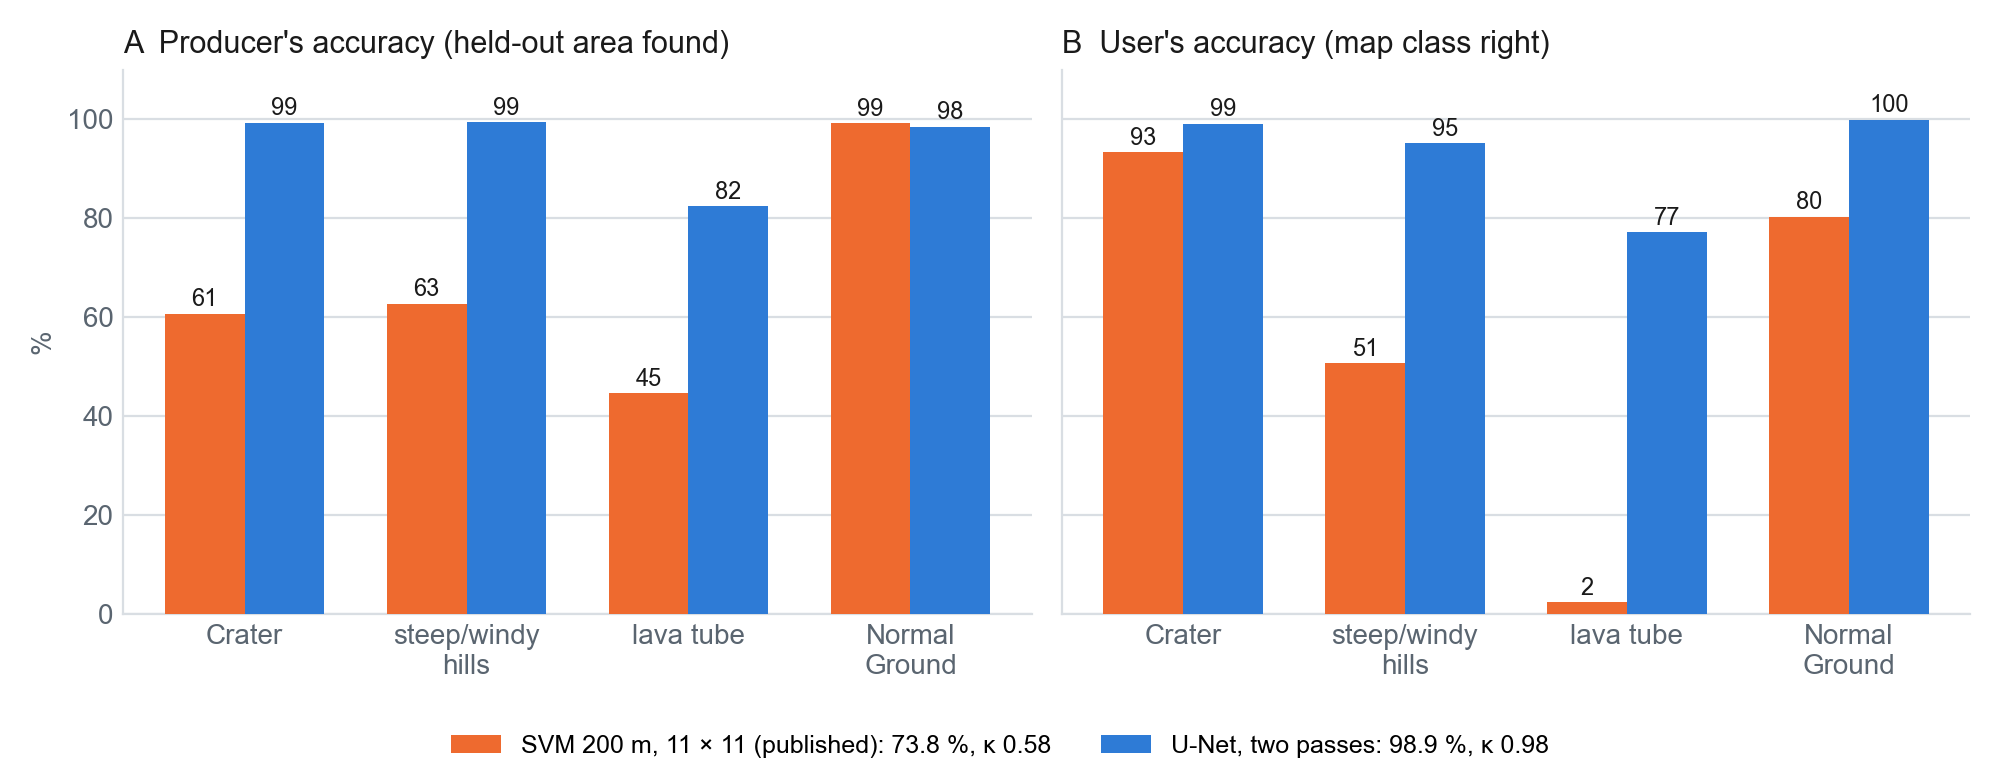
\includegraphics[width=\textwidth]{figures/svm_vs_unet.png}
\caption{The published support vector machine map and the two-pass U-Net map under the same scorer: producer's (A) and
user's (B) accuracy per class on the 183 held-out polygons. \label{fig:unet}}
\end{figure*}

%% ====================================================================================================
\section{Discussion} \label{sec:discussion}

\subsection{The hypotheses}

Table~\ref{tab:hyp} collects the verdicts. None of the four hypotheses is supported as stated. H3 failed outright: Iso
Cluster partitions trained on the west and east halves of Ius Chasma agree less for the four-band composite (adjusted
Rand index 0.40, \citealt{Hubert1985}) than for any single input (0.61 to 0.89), although the composite gives the most
coherent maps; a one-band clustering is close to a density slice and reproduces easily. H1 and H2 were tested on
stand-ins (map contacts and windows) and remain open for features digitised on the stack. %% KB §47.3, §47.5

\begin{table*}[t]
\centering
\caption{The hypotheses and tests \label{tab:hyp}}
\small
\begin{tabular}{llll}
\hline\hline
 & Claim & Verdict & Decisive number \\
\hline
H1 & Day IR shows flow margins Viking misses & not supported at 1:20\,M & day $-$ Viking $+8.7$ pt, interval $-1.7$ to $+18.1$ \\
H2 & Fluvial and volcanic channels separate & not supported at stage 1 & volcanic shallower; thermal AUC 0.50 \\
H3 & Composite classes are most stable & not supported & ARI 0.40 against 0.61--0.89 \\
H4 & Large IAU craters recovered & answered by fill depth & 68\% of 117 craters $\ge100$~km \\
T1 & Thermal IR improves the classification & yes, slightly & $+1.36$ and $+1.97$ pt, intervals above 0 \\
T3 & THEMIS tracks calibrated inertia & weakly, locally & within-block $|r|\approx0.1$; Viking $-0.36$ \\
T7 & Tributary orders resolved at 100~m & no DEM-supported answer & order follows threshold \\
\hline
\end{tabular}
\end{table*}

\subsection{Limits}

The central limit is in the data held. The THEMIS mosaics used here are display products, stretched region by region,
so they carry local contrast and texture; planet-wide material discrimination needs calibrated products such as the
TES inertia map, at the cost of resolution (3~km), or THEMIS-derived inertia \citep{Fergason2006} where it exists. In
this study the visible albedo carries the regional material signal.

The labels limit what the classification can show. The four hand-drawn classes are landforms, and slope and relief
alone predict them as well as the full stack; a test of thermal value needs material labels, which only photo
interpretation can give. Lava tube, with 44 polygons, is too thin a class for a planet-scale map; the U-Net makes it
usable only as a province.

An audit of the 512 labels found no two classes sharing ground, but five Crater polygons drawn around volcanoes (Arsia,
Pavonis and Ascraeus Mons, Tharsis and Ulysses Tholus) and six lava-tube polygons beside fluvial valleys. Arsia Mons
alone is 31\% of the held-out Crater area, so part of the Crater score, and of the U-Net's Crater province, measures
volcanic shields. A seven-class scheme follows from the audit: Crater narrowed to impact craters, with volcanic edifice,
apron and fluvial channel as new classes. Its 971 labels (734 training, 237 held out in the same 14 blocks) were
applied on 27 October. Every relabel, check and new edifice outline was reviewed by eye; the 172 apron and 276
fluvial-strip proposals were screened by a rule written before it ran (a strip kept only on a floor at least 20~m below
its flanks and off volcanic plains, an apron only where neither flat nor in a crater), not inspected one by one; and
hills fall short of the training minimum, in two training blocks against three. Both maps are scored on the same
held-out polygons, and the seven-class map replaces the published one only by a rule written before the run.
%% KB §68.1--§68.4, §69.8

The detectors are elevation-model products. Closed depressions miss breached craters by construction, and below about
5~km their density follows the sharpness of the HRSC/MOLA blend. Channels inherit the same dependence, and the fill
mask that removes synthetic lakes also breaks networks where the DEM is pitted.

The held-out test has been used once for each model. Any further tuning, of the deep-learning models above all, would
turn the 14 held-out blocks into a validation set; a next round needs validation blocks of its own. Finally, the manual
review of the 9,287 type-area candidates (2,610 and 3,283 channels, 1,685 and 1,709 depressions) has reached 549, all
at Ius Chasma, with a precision (accepts over accepts and rejects) of 54\% on the 188 steep, rock-floored channels and
7\% on 361 closed depressions. The
digitised classes hold 94 channels, 26 crater rims and no lava margins, so the machine products are presented as
candidates with measured recall and precision. %% KB §66.5, §6, §69.7, NEXT-STEPS §6

%% ====================================================================================================
\section{Conclusions} \label{sec:conclusions}

\begin{enumerate}
\item Four global products now share one co-registered grid over \pmsixty, 86.6\% of Mars, with the THEMIS pair never
resampled and the elevation model reproduced exactly at 200~m.
\item Visible albedo, day infrared and night infrared are three nearly independent dimensions locally, but the held THEMIS
mosaics carry local contrast only; calibrated thermal inertia follows Viking albedo across the planet.
\item Fill depth recovers 68\% of the large named craters and gives 465,354 closed depressions $\ge1$~km whose precision
against Robbins rises from 15.3\% to 62.2\% at 5~km; breached craters stay invisible.
\item Routed channels are dominated by the elevation model at \pmsixty\ (89.8\% under $2^{\circ}$), and stream order is a
parameter, not a measurement.
\item The published landform map scores 73.8\%, \kap\,0.58 on blocks it never saw; the thermal bands add a resolved 1.4
to 2.0 points. A U-Net reaches 98.9\% as a terrain-province map.
\item Lava flows are not separable in these bands; the geologic map remains the lava-flow reference, and H1 and H2 await
digitised margins and channels.
\end{enumerate}

\begin{acknowledgments}
This work was carried out for OCN~4704 Remote Sensing at the Florida Institute of Technology. The THEMIS mosaics are
products of the Arizona State University Mars Space Flight Facility; the Viking, HRSC/MOLA and geologic-map products are
distributed by the USGS Astrogeology Science Center; TES thermal inertia by the Planetary Science Institute; and the
crater database by S.~J.\ Robbins. The maps, scripts, trained models and derived rasters are archived at
\citet{Edwards2026data}.
\end{acknowledgments}

\facilities{Mars Odyssey (THEMIS), Viking Orbiter, MGS (MOLA, TES), Mars Express (HRSC)}

\software{ArcGIS Pro \citep{ArcGISPro}, GDAL \citep{GDAL}, NumPy \citep{Harris2020}, Matplotlib \citep{Hunter2007},
PyTorch \citep{Paszke2019}}

\bibliography{references}{}
\bibliographystyle{aasjournalv7}

\end{document}
